\documentclass[sigconf,review,anonymous]{acmart}

\makeatletter
\@ACM@balancetrue
\makeatother
\let\Bbbk\relax
\usepackage{amsmath,amssymb,mathtools}
\usepackage{amsthm}
\usepackage{booktabs}
\usepackage{multirow}
\usepackage{tabularx}
\usepackage{array}
\usepackage{float}
\usepackage{placeins}
\usepackage{tikz}
\usepackage{pgfplots}
\pgfplotsset{compat=1.18}
\usepackage{listings}
\usepackage{adjustbox}
\AtBeginDocument{%
  \setlength{\textfloatsep}{10pt plus 2pt minus 2pt}%
  \setlength{\intextsep}{9pt plus 2pt minus 2pt}%
  \setlength{\dbltextfloatsep}{12pt plus 2pt minus 2pt}%
}

% acmart pre-loads natbib, hyperref, xcolor, graphicx, microtype, geometry, fontenc, inputenc.
% Do not re-load them here.

\hfuzz=2pt
\emergencystretch=3em
\hbadness=10000
\vbadness=10000

\lstset{
  basicstyle=\ttfamily\footnotesize,
  breaklines=true,
  frame=single,
  language=Python,
  keywordstyle=\color{blue},
  commentstyle=\color{green!50!black},
  stringstyle=\color{red!70!black},
  showstringspaces=false
}

%==============================================================================
% ACM CONFERENCE METADATA
%==============================================================================
\acmConference[SACMAT '27]{The 32nd ACM Symposium on Access Control Models and Technologies}{June 2027}{To be announced}
\acmYear{2027}
\copyrightyear{2027}
\acmISBN{978-1-4503-XXXX-X/27/06}
\acmDOI{10.1145/XXXXXXX.XXXXXXX}
\setcopyright{acmlicensed}

%==============================================================================
% CCS CONCEPTS (REQUIRED BY ACM)
%==============================================================================
\begin{CCSXML}
<ccs2012>
   <concept>
       <concept_id>10002978.10003006.10003013</concept_id>
       <concept_desc>Security and privacy~Access control</concept_desc>
       <concept_significance>500</concept_significance>
       </concept>
   <concept>
       <concept_id>10002978.10003006.10003007</concept_id>
       <concept_desc>Security and privacy~Authorization</concept_desc>
       <concept_significance>300</concept_significance>
       </concept>
   <concept>
       <concept_id>10010147.10010178.10010224</concept_id>
       <concept_desc>Computing methodologies~Multi-agent systems</concept_desc>
       <concept_significance>300</concept_significance>
       </concept>
   <concept>
       <concept_id>10002978.10003001.10003003</concept_id>
       <concept_desc>Security and privacy~Logic and verification</concept_desc>
       <concept_significance>100</concept_significance>
       </concept>
 </ccs2012>
\end{CCSXML}

\ccsdesc[500]{Security and privacy~Access control}
\ccsdesc[300]{Security and privacy~Authorization}
\ccsdesc[300]{Computing methodologies~Multi-agent systems}
\ccsdesc[100]{Security and privacy~Logic and verification}

\keywords{access control, RBAC, ABAC, typed predicates, Model Context Protocol, agentic AI, LLM safety, policy enforcement, zero trust}

\title{PALADIN: Policy-Aware Layered Agentic Decision Intelligence over the Model Context Protocol}

%==============================================================================
% AUTHORS (ANONYMISED FOR DOUBLE-BLIND REVIEW)
%==============================================================================
% The "anonymous" class option suppresses author names, affiliations, and emails
% in the rendered PDF. Author metadata is retained below for the camera-ready.
\author{Author One}
\affiliation{%
  \institution{Anonymous Institution}
  \city{Anonymous City}
  \country{Anonymous Country}
}
\email{anon1@example.com}

\author{Author Two}
\affiliation{%
  \institution{Anonymous Institution}
  \city{Anonymous City}
  \country{Anonymous Country}
}
\email{anon2@example.com}

\author{Author Three}
\affiliation{%
  \institution{Anonymous Institution}
  \city{Anonymous City}
  \country{Anonymous Country}
}
\email{anon3@example.com}

\renewcommand{\shortauthors}{Anon.}

\begin{document}

%==============================================================================
% ABSTRACT
%==============================================================================
\begin{abstract}
\begin{sloppypar}
Autonomous LLM agents now invoke external tools through the Model Context Protocol (MCP), turning every tool call into an authorisation decision the protocol itself does not make. We argue this is an \emph{access-control} problem---and that the field has been answering the wrong question: \emph{semantic correctness is not authorisation correctness}. The tools that best accomplish a task can be exactly the ones an agent is not permitted to use, while a poorly-chosen bundle may be perfectly admissible. We introduce \textbf{PALADIN}, a deterministic invocation-time authorisation pipeline (SPIFFE/SPIRE identity, RBAC, ABAC, then TRAC), whose novel stage is \textbf{TRAC}---a \emph{task-relational} admission primitive that authorises an invocation on the coherence between the task and its proposed action-set.

Our central result: this deterministic floor holds worst-case security-failure rate to a fixed $10.3\%$, identical across every model---an invariance that holds \emph{by construction}, so what we measure is its \emph{magnitude}, not its model-independence. On ASTRA~\cite{elhelou2025astra}, an agentic tool-selection safety benchmark, six LLMs from three vendors used \emph{alone} as admission controllers wrongly admit $27$--$67\%$ of unsafe tool calls---unreliable, with no monotonic improvement across newer or stronger models. Composed \emph{behind} the floor, the \emph{same} models all converge to at most $7.3\%$. Around this we build a measurement framework for layered authorisation: it separates an LLM \emph{judging} a candidate bundle from one \emph{generating} it, and shows that na\"ive attribution misranks which policy layers matter. The floor guards \emph{semi-honest} mis-scoping (the common case) at a bounded false-block cost; it composes with prompt-injection defences for adversarial input and needs no bespoke runtime (verified OPA/Rego parity). All policies, logs, and scripts are released.
\end{sloppypar}
\end{abstract}

\maketitle

%==============================================================================
% SECTION 1: INTRODUCTION
%==============================================================================
\section{Introduction}
\label{sec:introduction}

\subsection{Motivation}
\label{sec:motivation}

LLM agents that autonomously select and invoke external tools have proliferated across enterprise and consumer domains~\cite{wang2024survey, xi2025rise}, building on tool-augmented language models~\cite{schick2023toolformer} and ReAct-style reasoning-and-acting loops~\cite{yao2023react}. They now standardise on the Model Context Protocol (MCP)~\cite{anthropic2024mcp} as the de facto tool-invocation interface. MCP deployments typically assume a trusted execution environment with no native identity verification, permission scoping, or deterministic predicate evaluation. The security gap is consequential: an agent tasked with ``investigating anomalous metrics'' might autonomously select tools that modify production alert rules, mutate database state, or initiate financial transactions far outside its intended mission. Recent analyses catalogue 16 MCP-lifecycle threat categories~\cite{gupta2025security} and document exploits including credential theft, tool poisoning, and remote code execution~\cite{jamshidi2025securing}.

Existing LLM-security work addresses fragments. Prompt-injection defences~\cite{liu2024formalizing, zhan2024injecagent} target adversarial reasoning manipulation; output filters such as Llama Guard~\cite{inan2023llamaguard} constrain generation content; agent-safety benchmarks~\cite{zhang2024agentsafetybench, yuan2024rjudge} evaluate behaviour in controlled environments. None reasons about the security properties of \emph{individual tool invocations} within a multi-domain operational context. Chu et al.~\cite{chu2026stateless} identify a layered attack-surface model but provide no enforcement mechanism; we instantiate one as a staged invocation-time pipeline.

This exposes a reframing the agentic-AC literature has largely missed: \emph{task-tool semantic correctness is not authorisation correctness}. A bundle a task-tool benchmark scores as ``correct''---the tools that best accomplish the task---may still be \emph{inadmissible} under the agent's role, attribute, and task-coherence constraints; conversely a benchmark-incorrect bundle may be perfectly admissible. Authorising agentic tool use is therefore an access-control problem, not a retrieval-accuracy one. It needs an enforcement primitive that conditions on the task$\leftrightarrow$bundle relation---a relation outside the \emph{conventional} attribute vocabulary of RBAC and ABAC, yet, like ReBAC and Purpose-BAC, enforceable on a standard policy engine once derived (\S\ref{sec:substrate_portability}).

\subsection{Contributions}
\label{sec:contributions}

Our primary contribution is an \emph{access-control} one: we recast agentic tool invocation as an authorisation problem (semantic correctness $\neq$ authorisation correctness) and introduce a \emph{task-relational} admission primitive---\textbf{TRAC} (task-relational access control)---that authorises on the discriminating signal conventional access control omits: the coherence between the task and its proposed action-set. We do \emph{not} claim a new formal model: TRAC needs no new rule-engine machinery and runs as rules-as-data on a commodity engine (verified OPA/Rego parity, \S\ref{sec:substrate_portability}). The novelty is the \emph{reframing}, the \emph{leak-free derivation} of that coherence attribute at invocation time (consuming no ground-truth label, \S\ref{sec:domain_inference}), a \emph{measurement methodology} for layered authorisation (how a deterministic policy stack and LLM judgement compose), and the empirical demonstration that measured semantic coherence is a reliable, load-bearing authorisation attribute---all realised in \textbf{PALADIN} (Policy-Aware Layered Agentic Decision Intelligence), our deterministic invocation-time authorisation pipeline (SPIFFE/SPIRE identity $\to$ RBAC $\to$ ABAC $\to$ a fact transformer $\to$ TRAC) in which TRAC is the novel stage. Concretely:

\begin{enumerate}
  \item A \textbf{methodology for measuring layered authorisation}: a dual-mode validation/selection protocol (the LLM \emph{judging} a candidate bundle vs.\ \emph{generating} one) that most benchmarks conflate; a single confusion-matrix convention (security $=$ precision, recall $=$ domain-eligible retention, with availability reported policy-conditioned) read at two resolutions---the model at \emph{task} resolution (positive $=$ correct) and the system at \emph{authorisation} resolution (positive $=$ valid), a gap that is itself diagnostic (\S\ref{sec:resolution_gap}); paired task-level bootstrap CIs on layer marginals; and a dataset-ceiling analysis bounding exact-match at $30$--$40\%$ (\S\ref{sec:methodology},~\ref{sec:conventions},~\ref{sec:resolution_gap},~\ref{sec:ceiling}).

  \item A \textbf{task-relational admission primitive, TRAC}: it authorises an invocation on the \emph{measured coherence between the task and the proposed bundle}---in-domain coverage, mutation safety, task--tool relevance---a task$\leftrightarrow$bundle relation not provisioned as a conventional RBAC/ABAC attribute and distinct from the workflow (TBAC~\cite{thomas1997tbac}), entity (ReBAC~\cite{fong2011rebac}), and \emph{declared}-purpose (Purpose-BAC~\cite{byun2005purpose}) axes. Derived by a fact transformer, it consumes \emph{no ground-truth label} (BM25 domain inference, \S\ref{sec:domain_inference}) and is enforceable on commodity engines (OPA/Rego parity, \S\ref{sec:substrate_portability}); we claim an empirical, load-bearing authorisation signal, not a new formal model. Every decision recomputes from the released logs without LLM calls.

  \item A \textbf{deterministic security floor whose \emph{magnitude} we measure}: conditioning on the bundle not the model, the stack returns a bit-identical profile (security-failure $10.3\%$, precision/security $0.63$, recall/retention $0.45$; policy-conditioned availability $0.81$) for every model---the empirical content is the floor's magnitude, not the by-construction invariance. Used \emph{alone}, the same models leak $27$--$67\%$ on the same inputs; composing the model's verdict behind the floor sharpens security-failure to $2.1\%$ (gpt-4o) and never exceeds the floor. A blind cross-vendor panel (Claude Opus 4.8, Sonnet 4.6, Gemini 2.5 Pro; all $6{,}942$ rows) converges to security-failure $\leq\!7.3\%$ (\S\ref{sec:stack_guarantee},~\ref{sec:newer_not_better}).

  \item \textbf{Complementary layers, measured two ways} (paired CIs): drop-one marginals are $-20.7$pp (RBAC) and $-12.0$pp (TRAC)---each individually load-bearing---while ABAC's is only $-0.9$pp (it overlaps RBAC) yet load-bearing when RBAC is absent (successive $-23.4$pp). Under a label defined independently of every policy artefact TRAC's marginal becomes the \emph{largest} (\S\ref{sec:reversal}); the successive/drop-one gap exposes a first-firing attribution pitfall (\S\ref{sec:per_domain}).

  \item \textbf{Attribution paradox and corroborated coverage}: (a) first-firing denial attribution misleads---RBAC claims $82\%$ of denials, yet ABAC (claiming $4\%$) carries the \emph{largest} successive marginal ($-23.4$pp)---a pitfall in much of the agent-safety literature; and (b) \emph{corroborated coverage} recovers legitimate work at near-zero security cost. We also reproduce ASTRA's LLM-ResM~\cite{elhelou2025astra} under a stricter per-bundle protocol (\S\ref{sec:attribution_paradox},~\ref{sec:corroborated}).
\end{enumerate}

\noindent\textbf{What this paper is not.} PALADIN is a security-first invocation-time floor, not an end-to-end agent-security solution: prompt-injection, tool-output exfiltration, MCP supply-chain, and side-channel attacks are out of scope and compose with it (\S\ref{sec:deployment_envelope}).

%==============================================================================
% SECTION 2: RELATED WORK
%==============================================================================
\section{Related Work}
\label{sec:related}

\subsection{Access Control, Policy Languages, and Task-Tool Benchmarks}
\label{sec:access_control}

Five decades of access-control foundations span lattice models~\cite{bell1973secure}, RBAC~\cite{sandhu1996role,ferraiolo2001proposed}, ABAC~\cite{hu2014guide}, and policy languages with decidable analysis (Cedar~\cite{cutler2024cedar}, XACML~\cite{oasis2013xacml}, Margrave~\cite{fisler2005verification}). These were designed for human principals on static boundaries; agents construct invocations dynamically via probabilistic reasoning and span multiple domains per task, producing tool bundles whose coherence with the task carries security-relevant signal.

Two AC lineages model structure beyond the subject and are the natural reference points for a ``task-relational'' claim. \emph{Task-Based Access Control} (TBAC)~\cite{thomas1997tbac} ties permission \emph{activation} to a task's workflow lifecycle---permissions are granted and revoked just-in-time as a task advances through its steps. \emph{Relationship-Based Access Control} (ReBAC)~\cite{fong2011rebac} authorises on \emph{relationships among entities} (owner-of, member-of, $\dots$). Our task-relational predicate is orthogonal to both: it gates on the \emph{semantic coherence between the task's intent and the proposed tool bundle}---is this bundle in-domain and sufficient for what the task asks?---not on a workflow position (TBAC) or an entity graph (ReBAC). It is complementary, not a replacement: an agent could be scoped by TBAC over a workflow \emph{and} checked by a task-relational coverage predicate at each invocation. Two further lineages sharpen the comparison: \emph{Purpose-Based Access Control}~\cite{byun2005purpose} authorises by the \emph{purpose} of an access---one the requester \emph{states} and the system validates only for \emph{entitlement to claim} (via conditional roles over role and system attributes), never for truthfulness---and \emph{Usage Control} (UCON)~\cite{park2004ucon} unifies authorisations, obligations, and conditions over mutable attributes with continuity of enforcement. TRAC differs in \emph{what} it conditions on: a \emph{measured} coherence between the task text and the proposed bundle, computed at invocation time from public tool descriptions---not a self-declared purpose label (which the semi-honest agent controls) nor an obligation model---and it composes with, rather than replaces, either.

Relative to Cedar and HashiCorp Sentinel---the substrates most often proposed for agentic authorisation---TRAC adds (i) typed predicates over \emph{derived} continuous relevance and coverage scores---BM25 task--domain and tool--task relevance over public metadata---with thresholds revisable as policy, (ii) a \emph{task-relational} coverage predicate---whether the proposed bundle covers the inferred task domain---conditioning on the task$\leftrightarrow$bundle relation rather than on caller or resource attributes alone, and (iii) bundle-level decision points composing over the full emitted tool set. We \emph{do} provide a head-to-head OPA/Rego re-implementation: the RBAC, ABAC, and TRAC layers run as rules-as-data on a standard Open Policy Agent runtime with decisions verified bit-identical to our reference engine (\S\ref{sec:substrate_portability}). This confirms our novelty is the task-relational \emph{predicate} and the measurement framework, not the rule engine---which is substrate-portable.

Could one of these methods be used \emph{instead} of the task-relational predicate? Not on this benchmark. The discriminating signal is the task$\leftrightarrow$bundle coherence, which lies outside the native vocabulary of every lineage above (subject, attribute, workflow, relationship, purpose, obligation). The policy \emph{engines}---Cedar, XACML, OPA/Rego, Sentinel (Margrave adds offline policy verification)---can \emph{host} such a predicate (we verify OPA/Rego decision parity, \S\ref{sec:substrate_portability}) but ship none themselves. So reusing any of them \emph{without} adding a measured coverage predicate leaves that signal unenforced and lands at the RBAC$\wedge$ABAC operating point---security-failure $0.223$ versus the full stack's $0.103$, a $2.2\times$ gap (Table~\ref{tab:factorial_ablation}) whose $+12$pp is precisely the predicate's marginal---so they are \emph{substrates or complements} for the predicate, not substitutes.

The closest task-tool benchmark is ASTRA~\cite{elhelou2025astra}, whose LLM reasoning matcher (LLM-ResM, per-tool GPT-4o with AND-aggregation) reports $F_1\!\approx\!0.67$ on the $N\!=\!3$ multi-tool test split. We re-use ASTRA's corpus and labels, reproduce LLM-ResM under a stricter per-bundle protocol (\S\ref{sec:astra_replication}), and evaluate what a deterministic stack composed on top achieves on the same inputs.

Concurrent with our work, the ASTRA team have extended their pipeline into a hybrid runtime framework, CASA~\cite{elhelou2026casa}, that pairs five \emph{deterministic} message-integrity checks (tool-definition, request-authorisation, action-alignment, parameter, and result-fidelity verification) with a two-stage \emph{semantic} layer---an LLM extracts the task from a multi-turn conversation, then an LLM judges each requested tool's relevance. This contemporaneous effort sharpens rather than pre-empts our contribution on three axes. First, their coherence signal is an \emph{LLM} per-tool judgment, whereas TRAC is a \emph{deterministic, leak-free} attribute derived from public metadata (\S\ref{sec:domain_inference}) and enforced as ordinary rules on an ABAC-class engine (\S\ref{sec:substrate_portability})---exactly the recomputable floor their own conclusion motivates when it observes that ``current semantic checks are not yet sufficient on their own'' for high-stakes tool use. Second, their deterministic checks govern \emph{message-flow integrity} (tampering, tool swaps, result falsification), which is orthogonal to---and composable with---our deterministic capability-\emph{coherence} envelope. Third, and most directly, CASA matches \emph{each tool independently} and explicitly lists bundle-level coherence---relevance that ``depends on the combination rather than individual tools''---as an \emph{open problem}; that combination is the set-valued task$\leftrightarrow$bundle relation TRAC gates (\S\ref{sec:trac}; bundle~D). Their genuine advance over prior work---multi-turn task \emph{extraction} from conversational context---is complementary to, and outside the scope of, our single-task, persona-grounded setting; and unlike their extractor, which trusts the recovered task, we assume a \emph{semi-honest} agent whose declared purpose cannot be trusted (\S\ref{sec:threat_model}).

\subsection{Zero-Trust, Agent Identity, and MCP Security}
\label{sec:zero_trust}
\label{sec:agent_safety}

NIST Zero Trust~\cite{rose2020zero} and SPIFFE~\cite{spiffe2022} establish cryptographic workload identity but have not been applied to AI-agent identity; recent delegation work~\cite{south2025authenticated,rampalli2026pedigree} and defence-in-depth surveys~\cite{chu2026stateless,jangam2024comprehensive,muhammad2024integrative} map the layered attack surface without providing formal enforcement.

The agent-safety community has produced evaluation frameworks---Agent-SafetyBench~\cite{zhang2024agentsafetybench}, ToolEmu~\cite{ruan2024toolemu}, GuardAgent~\cite{xiang2024guardagent}, R-Judge~\cite{yuan2024rjudge}, ALMITA~\cite{arcadinho2024almita}, Constitutional AI~\cite{bai2022constitutional}, deceptive-alignment analyses~\cite{hubinger2024sleeper}---and prompt-injection defences~\cite{liu2024formalizing,zhan2024injecagent,debenedetti2024agentdojo,kim2025promptflow,inan2023llamaguard}. These treat the agent monolithically and do not enforce authorisation at the invocation boundary. MCP-specific work has begun mapping the landscape (16 threat categories~\cite{gupta2025security}, practical exploits~\cite{jamshidi2025securing}, cross-server tool poisoning~\cite{invariantlabs2025toolpoisoning}); multi-agent and behavioural-trust efforts~\cite{patil2026sentinelagent,schroederdewitt2025open,xu2025master,wu2023autogen,rao1995bdi,csa2025fortifying,cisco2025redefining} establish the problem space but offer ad-hoc rather than staged enforcement. Foundational tool-augmented architectures~\cite{schick2023toolformer,yao2023react,wang2023voyager,wang2024survey,xi2025rise} provide the agents but no governance for their invocations; PALADIN is architecture-agnostic and composes on top.

%==============================================================================
% SECTION 3: THE PALADIN PIPELINE
%==============================================================================
\section{The PALADIN Pipeline}
\label{sec:architecture}
\label{sec:framework}


PALADIN authorises each tool invocation through an ordered stack of deterministic gates that culminates in TRAC. We first fix the admission model and its short-circuit algebra (\S\ref{sec:state_model}), state the threat model (\S\ref{sec:threat_model}), give the design rationale and walk a single request through the pipeline (\S\ref{sec:pipeline_overview}), then develop the conventional layers (\S\ref{sec:layers}) and, as the novel stage, TRAC (\S\ref{sec:trac}).

\subsection{Gate Control and Short-Circuit Composition}
\label{sec:state_model}
\label{sec:request_model}
\label{sec:composition}
\label{sec:composition_properties}


A tool invocation request is modelled as a 5-tuple
\begin{equation}
r = \langle \iota, \tau, T, M, \delta \rangle
\label{eq:request}
\end{equation}
where $\iota$ is the agent identity (SPIFFE ID), $\tau$ the task description, $T=\{t_1,\dots,t_n\}$ and $M=\{m_1,\dots,m_n\}$ the selected tools and their MCP servers, and $\delta$ the environmental context (timestamp, compliance tier).

\paragraph{Unit of decision: a per-invocation reference monitor.} $\Pi$ is a reference monitor at the MCP invocation boundary: it authorises \emph{each request} $r$ at the moment the agent emits it, as an operating system mediates each system call---not a single up-front verdict over a whole task. A request carries the task $\tau$ as trusted provenance (\S\ref{sec:threat_model}) together with the tool(s) invoked at that step---one tool in the common case, or the small set an agent emits in a single step (what the evaluation corpus supplies per task, our unit of evaluation). The agent never declares its whole task in advance and $\Pi$ never enumerates future requests: because $\tau$ is present at \emph{every} step, $S_6$ can judge whether \emph{this} step coheres with the mission without foreknowledge of later ones. Admission is therefore incremental---an agent whose in-domain reads are admitted keeps making progress while a single out-of-scope call (a cross-domain write, say) is denied, after which it re-plans and completes the task through admitted calls. Stages $S_1$--$S_4$ evaluate the classical subject/object/operation triple over the tool invocation $(\iota,(t,m),a(t))$; $S_6$ adds one object conventional access control does not name---the capability the bundle exercises \emph{in service of} $\tau$ (\S\ref{sec:stage_definitions}). What $\Pi$ mediates is that invocation boundary---which capability an agent may exercise---not the internal objects of the remote service, whose own access control composes with, and is out of scope for, this layer. \S\ref{sec:worked_example} traces a concrete request end-to-end.

The short-circuit composition operator $\rhd$ between stages is
\begin{equation}
\begin{aligned}
(S_i \rhd S_j)(r) &= \\
&\begin{cases}
\text{DENY}_i, & \text{if } S_i(r) = \text{DENY}, \\
S_j(r), & \text{otherwise.}
\end{cases}
\end{aligned}
\label{eq:composition}
\end{equation}
$S_5$ is not a decision stage but a deterministic \emph{fact-transformer} $\phi\!:\!r\!\mapsto\!\Phi(r)$ that materialises the typed fact base consumed by $S_6$; it cannot return DENY. The full pipeline is therefore
\begin{equation}
\Pi(r) = \bigl(S_1 \rhd S_2 \rhd S_3 \rhd S_4 \rhd S_6\bigr)\!\bigl(r,\phi(r)\bigr),
\label{eq:pipeline}
\end{equation}
i.e. $\phi$ runs once when $S_1$--$S_4$ all admit, and $S_6$'s predicates evaluate over $\Phi(r)$.

Each stage records \texttt{ALLOW}, \texttt{DENY}, or \texttt{NOT\_EVALUATED}; the final decision is the conjunction of evaluated stages. A \texttt{DecisionResult} carries the per-stage map, final decision (\texttt{ALLOW}/\texttt{DENY}), denial source, and audit trace. Short-circuiting yields three benefits: computational efficiency (S6 is skipped when cheaper checks suffice), security hardening (later stages cannot mask upstream denials), and audit clarity (the denial source unambiguously identifies the triggering concern).

Beyond the per-stage states, the pipeline returns a single binary admission decision: $\Pi(r)=\text{ALLOW}$ only if every evaluated stage allows, and $\text{DENY}$ otherwise. There is no third outcome---a denied high-risk write simply stays \texttt{DENY}---which keeps every layer expressible as a standard ALLOW/DENY policy (\S\ref{sec:substrate_portability}). Advisory TRAC rules (\S\ref{sec:trac}) may additionally raise non-blocking alerts on an admitted bundle, but these never change the admission decision and are excluded from the security metrics.

The operator $\rhd$ gives $\Pi$ three properties. \textbf{(P1) Monotonicity:} adding a stage can only convert ALLOW to DENY (immediate from the short-circuit semantics). \textbf{(P2) Order-independence of unique necessity:} if a single $S_k$ is the only stage that would deny $r$, $\Pi(r)=\mathrm{DENY}$ regardless of ordering. \textbf{(P3) Fail-secure default:} predicates default conservatively on missing facts and stage exceptions are wrapped to DENY, so partial failure cannot silently degrade to ALLOW. P1 grounds the $\Delta$-value reading; P2 underpins the attribution analysis (\S\ref{sec:attribution_paradox}).

\subsection{Threat Model and Deployment Envelope}
\label{sec:threat_model}


\textbf{Adversary.} A \emph{semi-honest agent}: an authenticated LLM-driven workload that, given an operator- or workflow-supplied task, may select and emit a tool bundle that exceeds scope, crosses domains, targets writes without prior reads, or otherwise violates policy---through hallucination or over-helpful, helpfulness-optimised behaviour. It controls the \emph{emitted bundle}; the task text is trusted provenance (operator/workflow), which is what makes the task-relational predicates meaningful. Active manipulation of the task text itself---prompt injection \emph{into the task}, crafted to steer the relevance predicates---is out of scope and composes with the prompt-injection defences of \S\ref{sec:deployment_envelope}.

\textbf{Trust assumptions.} We trust the SPIFFE/SPIRE identity substrate \emph{and the mutual-TLS transport it anchors} (\S\ref{sec:layers}), policy YAML/JSON integrity at load, the MCP tool registry, and the deterministic pipeline; we do \emph{not} trust LLM-emitted bundles or natural-language justifications, and we admit \emph{no} self-reported model confidence as a policy input---every score TRAC thresholds is recomputed deterministically from public metadata and the trusted task text (\S\ref{sec:domain_inference}).

\textbf{In-scope.} Within-domain mis-scoping, cross-domain capability leakage, mutation-without-read, hard-capability gaps, and trust-state misalignments (operationalised by the evaluation dataset's \texttt{wrong}/\texttt{null} negatives). \textbf{Out of scope:} policy-file compromise, side channels, DoS, MCP supply-chain attacks, active adversarial prompts crafted to evade specific predicates, and tool-output exfiltration. \textbf{Security objective:} minimise the security-failure rate (Eq.~\ref{eq:secfail}) subject to a bounded false-block rate on admissible requests; the trade-off point is set by policy, not architecture.

\textbf{Deployment envelope.} PALADIN is an invocation-time authorisation layer, not an end-to-end agent-security solution. The exclusions above are not minor: each is an active research area, and production deployment composes PALADIN with output filters (e.g., Llama Guard~\cite{inan2023llamaguard}), signed registries, network-layer rate limiting, and prompt-injection defences~\cite{liu2024formalizing}. Contribution claims are scoped to that envelope. TRAC's two enforcing predicates are deterministic relevance controls over the task text, so its deterministic guarantee targets \emph{semi-honest} mis-scoping---hallucination, over-helpfulness, and benign scoping errors (the evaluation dataset's non-adversarial \texttt{wrong}/\texttt{null} negatives), the dominant failure mode of today's agents. Active task-text manipulation---an adversary crafting wording to lexically match a target bundle---is owned by trusted task provenance and the composed prompt-injection controls above, not by this layer.

\subsection{Design Rationale and Pipeline Overview}
\label{sec:design_rationale}
\label{sec:pipeline_overview}

PALADIN is assembled from a small set of security principles, each realised by one mechanism in the stack (Table~\ref{tab:rationale}). The design is deliberately \emph{layered and deterministic}: independent concerns are separated into stages that each admit or deny for one auditable reason, and the only non-deterministic decider---an optional LLM verdict---is confined so that it can never weaken the guarantee.

\begin{table}[!t]
\centering
\caption{PALADIN's design principles, the mechanism realising each, and why it is needed. Several are consolidated from properties stated where they are first used (short-circuit benefits, \S\ref{sec:state_model}; fail-secure and monotonicity, \S\ref{sec:composition_properties}; substrate portability, \S\ref{sec:substrate_portability}). The optional LLM verdict gate ($G$) is listed as a first-class layer, confined so it can only add denials.}
\label{tab:rationale}
\footnotesize
\begin{adjustbox}{max width=\columnwidth}
\begin{tabular}{@{}lll@{}}
\toprule
\textbf{Principle} & \textbf{Mechanism} & \textbf{Why} \\
\midrule
Zero-trust identity & $S_1$ SPIFFE/SPIRE + mTLS & MCP assumes a trusted host; verify the agent and the channel, do not trust the caller \\
Closed-world tools & $S_2$ registry & admit only registered tools; unknown/poisoned servers cannot be invoked \\
Least privilege (role) & $S_3$ RBAC & an agent gets only the (domain, tool) pairs its persona needs \\
Context-sensitive gates & $S_4$ ABAC & clearance/trust/department/risk conditions a role cannot express \\
Leak-free, replayable facts & $S_5$ transformer $\phi$ & decisions recompute from logs with no LLM call and no ground-truth label \\
Task-relational least privilege & $S_6$ TRAC & authorised $\neq$ coherent: catch hallucinated/over-helpful bundles $S_3$--$S_4$ admit \\
Optional model second-opinion & $G$ LLM verdict (validation) & a conjunctive gate behind the floor: can only \emph{add} denials, never admit what the floor denies \\
Fail-secure default & all stages (P3) & missing facts and stage exceptions resolve to DENY \\
Cheap-to-costly ordering & short-circuit $\rhd$ & set-membership first, fact-derivation last: efficiency, no masking, audit clarity \\
Substrate portability & rules-as-data & commodity engines (OPA/Rego parity) reproduce every decision \\
\bottomrule
\end{tabular}
\end{adjustbox}
\end{table}

\textbf{Why this order.} Stages are ordered by increasing cost and decreasing certainty. The cheapest, most certain checks---cryptographic identity and registry membership---run first; role and attribute policy follow; the costliest signal, the leak-free relevance-and-domain fact derivation that $S_6$ consumes, runs \emph{only} once every cheaper stage has admitted (Eq.~\ref{eq:pipeline}). Short-circuit composition then guarantees that a later, more permissive-looking stage can never overturn an upstream denial (monotonicity, P1, \S\ref{sec:composition_properties}) and that the denial source is unambiguous for audit (\S\ref{sec:state_model}).

\textbf{Why a deterministic floor, then an optional model verdict.} The deterministic stages are model-independent and recomputable from the released logs; the LLM verdict, when present (validation mode), composes \emph{conjunctively} behind them (FULL $=$ floor $\wedge$ verdict), so it can only \emph{add} denials, never admit what the floor denies. This bounds the trusted computing base to the deterministic stack and keeps the model out of the decision's integrity: a compromised or hallucinating verdict degrades permissiveness, not security (\S\ref{sec:threat_model}).

\textbf{Why facts precede rules.} Separating fact derivation ($\phi=S_5$) from predicate evaluation ($S_6$) makes every task-relational decision a pure function of typed facts. The same $\Phi(r)$ yields the same, individually explained verdict on replay, and the rules---being data over derived attributes---port unchanged to a commodity policy engine (\S\ref{sec:substrate_portability}).

\textbf{Pipeline realisation.} The Unified Decision Engine executes these principles as six sequential stages with short-circuit semantics: any \texttt{DENY} from stages S1--S4 terminates the pipeline immediately (Figure~\ref{fig:pipeline}). S5 extracts typed facts; S6 (TRAC) consumes them for predicate-level evaluation; in \emph{validation} mode an optional LLM verdict gate $G$ then composes conjunctively behind $S_6$.

\textbf{Two evaluation modes.} We exercise this pipeline in two complementary modes that differ \emph{only} in where the proposed tool bundle originates; the six deterministic stages are identical in both (full protocol in \S\ref{sec:dual_mode}). In \emph{validation} mode the LLM is handed the task \emph{and} a candidate bundle and returns the admit/deny \emph{verdict} $G$ of Figure~\ref{fig:pipeline}. In \emph{selection} mode the LLM is given the task \emph{alone} and must \emph{generate} the bundle, which is then routed through the \emph{same} deterministic stages with no verdict gate. The two modes isolate the two ways an LLM can fail an authorisation---mis-\emph{judging} a bundle it is shown versus mis-\emph{selecting} the bundle it emits---and let us show that the same deterministic floor recovers both (\S\ref{sec:whole_flow}).

\begin{figure}[!t]
\centering
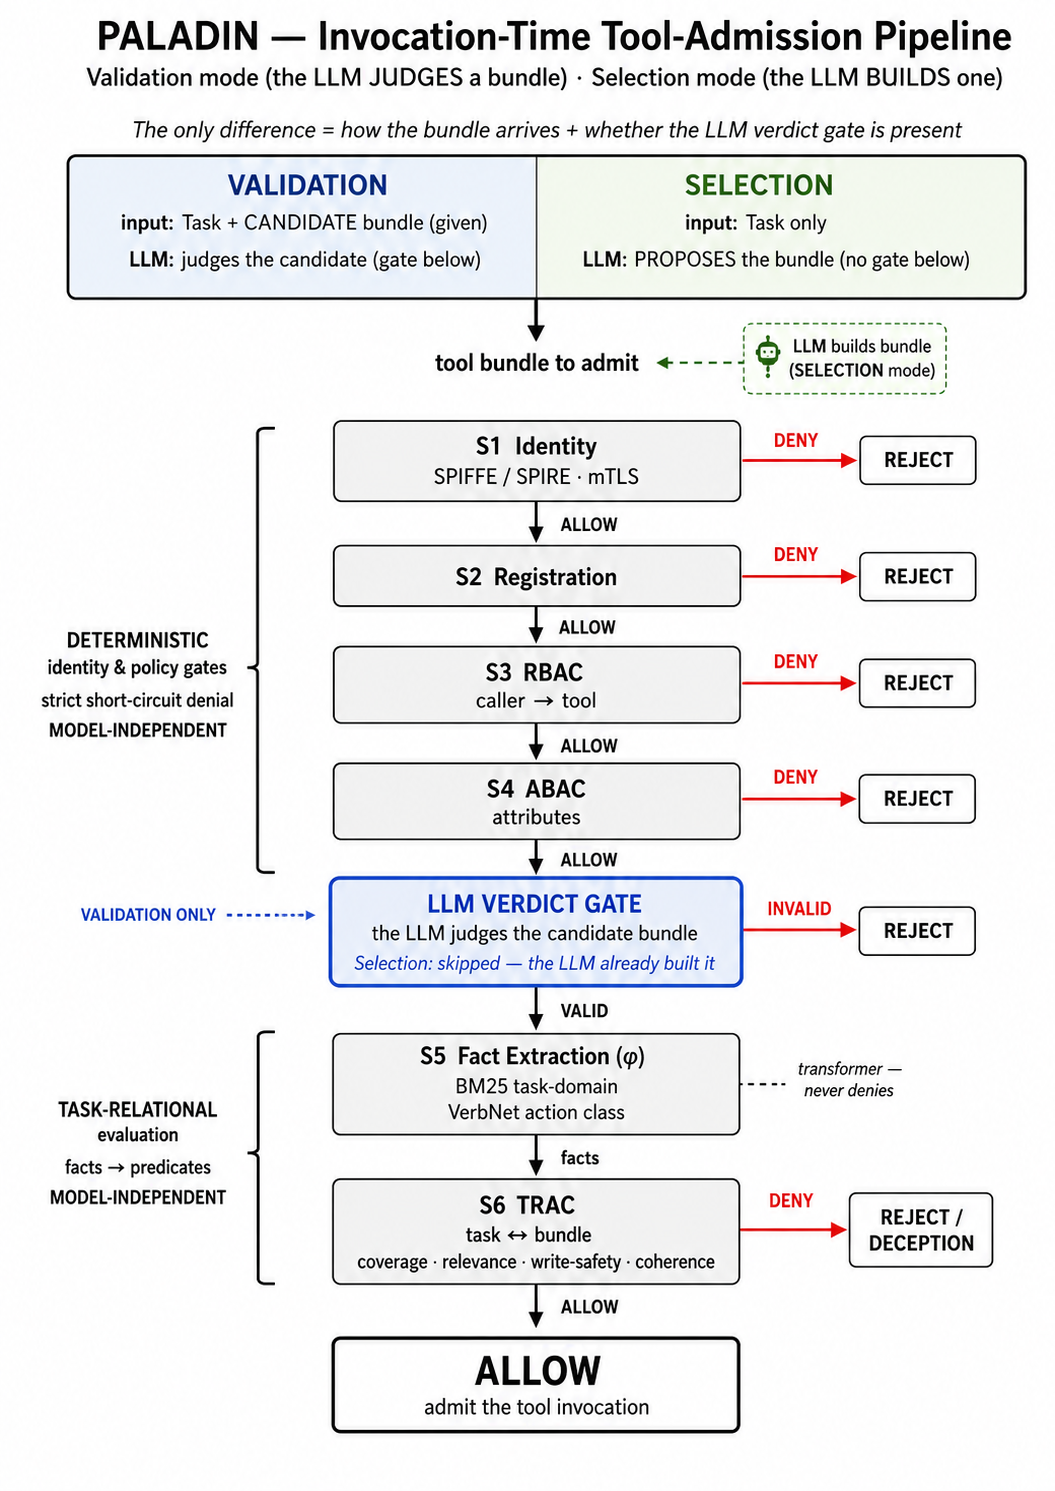
\includegraphics[width=0.8\columnwidth]{figures/pf1.png}
\caption{PALADIN's six‑stage admission pipeline (short‑circuit S1–S4; S5 fact transformer → S6 TRAC). The deterministic stages are model‑independent; the LLM verdict gate composes \emph{conjunctively} with the deterministic floor (its drawn position is presentational---FULL $=$ floor $\wedge$ verdict) and is present only in validation, while in selection the LLM instead generates the bundle.}
\Description{Flow diagram showing an MCP tool request passing through identity, registration, RBAC, ABAC, fact extraction, and TRAC stages before allow or deny.}
\label{fig:pipeline}
\end{figure}

Table~\ref{tab:soo} names the classical access-control triple---subject, object, operation---that each \emph{deciding} stage evaluates, with its admission condition, and adds the LLM as its one non-deterministic component. We list only components that render an access-control verdict: authentication ($S_1$) \emph{establishes} the subject rather than authorising an access, and the fact transformer ($S_5$) materialises $\Phi(r)$ without deciding, so neither is a row (both are detailed in \S\ref{sec:layers}). $S_2$--$S_4$ are a standard reference monitor over the tool invocation; ABAC ($S_4$) reuses the \emph{same} subject and object as RBAC and merely adds attributes to the policy. $S_6$ is the one \emph{deterministic} stage whose object---the capability the bundle exercises in service of the task---is not an attribute RBAC or ABAC \emph{provisions}, but a relation over the task and the whole bundle that must be \emph{derived} (\S\ref{sec:why_not_abac}); the LLM's role is mode-dependent---in validation it is the gate $G$, an \emph{optional} second opinion behind $S_6$; in selection the same model instead \emph{generates} the bundle the deterministic stages decide.

\begin{table}[!t]
\centering
\caption{The subject, object, and operation each \emph{deciding} stage evaluates, with its admission condition. Only genuine access-control stages appear: authentication ($S_1$) establishes the subject, and the fact transformer ($S_5$, $\phi$) renders no verdict, so neither is a row (both in \S\ref{sec:layers}). $S_2$--$S_4$ form a classical reference monitor over the invocation $(\iota,(t,m),a(t))$; ABAC ($S_4$) uses the \emph{same} subject and object as RBAC, adding subject-, resource-, action-, and environment-\emph{attributes} to the policy. $S_6$'s object---the capability the bundle exercises in service of $\tau$---is not an attribute RBAC or ABAC \emph{provisions} but a \emph{derived} relation over $\tau$ and the whole bundle (\S\ref{sec:why_not_abac}). The LLM (last row) has a \emph{mode-dependent} role: in \emph{validation} it is the gate $G$---the one \emph{non-deterministic} decider---composing conjunctively behind $S_6$ (FULL $=$ floor $\wedge$ verdict) so it can only add denials; in \emph{selection} the \emph{same} model instead \emph{generates} the object (the candidate bundle) that $S_2$--$S_6$ decide, rendering no verdict of its own.}
\label{tab:soo}
\footnotesize
\begin{adjustbox}{max width=\columnwidth}
\begin{tabular}{@{}lllll@{}}
\toprule
\textbf{Stage} & \textbf{Subject} & \textbf{Object} & \textbf{Operation} & \textbf{Admits iff} \\
\midrule
$S_2$ Registration & agent & tool$@$server $(t,m)$ & invoke & every $(t,m)$ registered \\
$S_3$ RBAC         & role $\rho(\iota)$ & (domain, tool) & invoke as $a(t)$ & $(m,t)\in\rho(\iota)$ \\
$S_4$ ABAC         & agent \emph{(+attrs)} & resource \emph{(+attrs)} & read/write/destructive & subject/resource/env attributes permit \\
$S_6$ TRAC         & agent & capability set for $\tau$ & exercise bundle for $\tau$ & bundle coheres with $\tau$ \\
$G$ LLM \emph{(val./sel.)} & agent & bundle for $\tau$ & judge \emph{(val.)} / generate \emph{(sel.)} & \emph{val.:} bundle consistent with $\tau$; \emph{sel.:} model emits it \\
\bottomrule
\end{tabular}
\end{adjustbox}
\end{table}

\subsection{Conventional Layers: Identity, Registration, RBAC, and ABAC}
\label{sec:layers}
\label{sec:stage_definitions}
\label{sec:rbac_abac_classification}
\label{sec:identity}


This section derives the typed predicates each layer consumes---from persona-scoped RBAC grants and attribute rules, through the read/write action classes inferred from tool metadata, to the task-relational facts TRAC evaluates.

\textbf{S1--S2} are deterministic set-membership checks: $S_1$ admits iff $\iota \in \mathcal{I}_{\text{valid}}$, and $S_2$ admits iff every $t\in T$ is in the registry $\mathcal{R}(m_t)$. \textbf{S3 (RBAC)} evaluates role-based permissions:
\begin{equation}
S_3(r) = \begin{cases}
\text{ALLOW} & \text{if } \forall (m_j, t_j) \in \text{zip}(M,T)\!: (m_j, t_j) \in \rho(\iota) \\
\text{DENY} & \text{otherwise}
\end{cases}
\label{eq:rbac}
\end{equation}
where $\rho(\iota)$ maps an identity to its permitted (domain, tool) pairs. \textbf{S4 (ABAC)} implements first-match semantics over attribute conditions,
\begin{equation}
S_4(r) = \text{first-match}(\mathcal{P}_{\text{ABAC}}, \text{attrs}(r)),
\label{eq:abac}
\end{equation}
with $\mathcal{P}_{\text{ABAC}}$ the ordered policy set and $\text{attrs}(r)$ extracting subject, resource, action, and environment attributes. \textbf{S5} is the fact-transformer $\phi$ of Eq.~\ref{eq:pipeline}: it derives typed facts without making any decision. 

\textbf{Agent-adapted RBAC} maps agent personas to permissions over tool bundles across MCP domains, with three adaptations from traditional RBAC: tool-level granularity (per individual tool rather than per service endpoint); wildcard domain grants for trusted agents (e.g., \texttt{grafana.*}); and cross-domain permission intersection requiring permissions in \emph{all} referenced domains across dynamically-constructed multi-tool bundles.

\textbf{ABAC} first-matches an ordered rule set over the subject, resource, action, and environment attributes of the request (\S\ref{sec:stage_definitions}). The released ruleset contains $6$ rules in three families, conditioning on \emph{subject} (department, clearance level, trust score), \emph{resource} (compliance tier, data sensitivity, risk level), and \emph{action} (write, destructive-write) attributes: \emph{department/compliance isolation} (Financial/PCI-DSS resources restricted to Finance; Infrastructure writes to Engineering or Infrastructure), \emph{clearance gates} (L2 to read high-risk resources, L3 to write them, L3 for destructive operations), and a \emph{trust gate} (trust score $\geq 0.8$ to write). A rule denies when all its conditions hold; conditions fail closed on an absent attribute; the request is denied if any rule fires.

\textbf{Action classification.} Each tool's action class $a(t)\in\{\textrm{read},\textrm{write}\}$ (\texttt{destructive} a write subtype) is derived deterministically from the two universally-available MCP fields---tool \emph{name} and \emph{description}---by a verb lexicon grounded in established verb classes (Levin's verb classes~\cite{levin1993verbs}, catalogued in VerbNet~\cite{schuler2005verbnet}) mapped to a read/write/destructive taxonomy (CRUD; RFC~9110 safe/unsafe methods). The leading description verb is lemmatised and class-mapped, ambiguous verbs are read-guarded (\emph{run/execute a query} $\to$ read), and the tool name escalates only toward write/destructive (fail-safe defaults). There is no curated per-tool label map. Request-level predicates follow by composition---$\text{ContainsWrite} = \bigvee_{t \in T} (a(t)=\texttt{write})$, and analogously $\text{ContainsDelete}$ and $\text{ContainsRead}$---and become typed inputs to TRAC.

\textbf{Agnostic capability.} The capability a tool provides is the pair $\{d(t)\}{:}\{a(t)\}$ of \S\ref{sec:capability}---its MCP domain $d(t)$ and the action class $a(t)$ above---with the subsumption $\{d\}{:}\textrm{write}\sqsupseteq\{d\}{:}\textrm{read}$. There is \emph{no} capability catalog, entailment ontology, or hard/soft capability tier: coverage is the single domain floor of Eq.~\ref{eq:hardcap}, evaluated against the BM25-inferred task domain (\S\ref{sec:domain_inference}), while mutation- and relevance-level concerns are delegated to the \texttt{write\_safety} and \texttt{tool\_relevance} rules (\S\ref{sec:trac}). The model therefore consumes no per-MCP vocabulary, no curated tool$\to$capability map, and no ground-truth label---the property that makes the pipeline leak-free.

\paragraph{Identity infrastructure.} PALADIN uses cryptographic agent identity (SPIFFE/SPIRE) as the source of $\iota$ in the request tuple (\S\ref{sec:request_model}); identity is an \emph{input} to the policy stack, not itself a contribution we evaluate. Each agent receives a SPIFFE ID encoding role and trust attributes (clearance, department, trust score); SPIRE issues SVIDs with automatic rotation and workload-selector attestation. We do not measure rotation overhead, attestation failure modes, or delegation-substrate properties; that work belongs to identity-infrastructure literature~\cite{rampalli2026pedigree,south2025authenticated}, over which PEDIGREE-style multi-hop delegation could compose. Persona-to-domain allow-lists are released with the artefact.

\paragraph{Transport authentication (mTLS).} The same SPIRE-issued identities anchor the transport. Each workload presents its X.509 SVID to establish \emph{mutual} TLS with the MCP invocation boundary, so both endpoints are cryptographically authenticated and every request travels an encrypted, identity-bound channel---the transport half of stage $S_1$ (Fig.~\ref{fig:pipeline}). This is the transport realisation of zero-trust identity: the caller is trusted by neither network position nor a bearer token, but by a rotating certificate bound to its workload identity. Like the identity substrate itself, mTLS is trusted pass-through---we assume it and do not measure it; certificate issuance, rotation, and revocation are handled by SPIRE and lie outside the authorisation results. Folding it into $S_1$ keeps the model at six numbered stages (Fig.~\ref{fig:pipeline}) while making explicit that authentication covers both \emph{who} the agent is and the \emph{channel} its invocation rides.

\subsection{TRAC: a Task-Relational Admission Primitive}
\label{sec:trac}
\label{sec:capability}
\label{sec:alignment}


\textbf{S6 (TRAC)} evaluates typed predicates over $\Phi(r)$:
\begin{equation}
S_6(r) = \begin{cases}
\text{DENY} & \text{if } \exists\, R_i \text{ s.t. } \text{triggered}(R_i) \land a_i = \text{DENY} \\
\text{ALLOW} & \text{otherwise.}
\end{cases}
\label{eq:trac}
\end{equation}

TRAC's capability model is deliberately \emph{agnostic}: a capability is the pair $\{d\}{:}\{a\}$, where $d$ is the MCP a tool belongs to and $a\in\{\textrm{read},\textrm{write}\}$ is its action class, with the subsumption rule that a write also grants the read ($\{d\}{:}\textrm{write}\sqsupseteq\{d\}{:}\textrm{read}$). There is no per-MCP vocabulary, no capability catalog, and no curated tool$\to$capability map: the bundle's provided capabilities are $\mathrm{HasCap}=\{\{d(t)\}{:}\{a(t)\}\mid t\in T\}$, derived mechanically from each tool's MCP and its read/write class (\S\ref{sec:layers}). Coverage is domain-only: the required capability for a task with inferred domain $d_\tau$ is the action floor $\{d_\tau\}{:}\textrm{read}$---any in-domain tool, read or write, satisfies it---and a hard violation is
\begin{equation}
\mathrm{HardCapMissing}(r)\;\triangleq\;\{d_\tau\}{:}\textrm{read}\notin\mathrm{HasCap}.
\label{eq:hardcap}
\end{equation}
We deliberately do \emph{not} infer read-vs-write \emph{intent} from task text, nor gate on a weighted alignment score: those heuristics were substring-fragile and, for the domain signal, oracle-dependent. Mutation concerns are owned by the \texttt{write\_safety} advisory and lexical task--bundle fit by \texttt{tool\_relevance} (\S\ref{sec:trac}). $d_\tau$ itself is inferred from the task text alone (\S\ref{sec:domain_inference}), so the entire coverage check is free of any ground-truth label. This is a property conventional RBAC (caller$\to$tool) and ABAC do not \emph{provision} as a standard, trusted attribute: whether the proposed bundle is coherent with the task's domain---expressible, as we show, over \emph{derived} attributes on a standard engine (\S\ref{sec:substrate_portability}, \S\ref{sec:why_not_abac}).

TRAC (Task-Relational Access Control) conditions admission on the \emph{measured relation between the task and the proposed tool bundle}---in-domain coverage, mutation safety, and task--tool relevance---which conventional RBAC (caller$\to$tool) and ABAC do not \emph{provision} as a standard attribute, and which is distinct from the TBAC/ReBAC/Purpose-BAC axes (\S\ref{sec:related}, \S\ref{sec:why_not_abac}). We claim no new formal model: the contribution is empirical---identifying, enforcing, and measuring this relation as a load-bearing signal---enforceable on commodity engines. Its expressive content equals a typed Cedar~\cite{cutler2024cedar} or OPA/Rego extension with custom builtins for continuous LLM-emitted scores; an OPA/Rego re-implementation of the identical rules-as-data reproduces every decision (\S\ref{sec:substrate_portability}), leaving only the substrate's \emph{performance} cost to benchmark. The engine is \emph{typed} (booleans, enums, reals), \emph{staged} (facts derived in $\phi=S_5$ before any $S_6$ rule fires), \emph{ordered} (enforcing rules short-circuit on the first denial), and \emph{partitioned} into \emph{enforcing} rules (change ALLOW/DENY) and \emph{advisory} alert-only rules (Table~\ref{tab:trac_rules}); evaluation is $O(n)$ given pre-computed facts.

\emph{Scope.} TRAC is a \emph{capability-envelope} check---does the domain$\times$action a bundle would exercise fall within the task's inferred domain?---not a prediction of whether a call is \emph{safe} or a tool \emph{benign}. It is thus \emph{necessary, not sufficient}: an in-domain bundle can still misbehave, and clearing TRAC scopes an invocation without vouching for it. This is deliberate. Deciding whether an arbitrary, possibly-malicious payload is safe to execute from its metadata alone is not an access-control question and is intractable in general; TRAC instead gates the one static, decidable property that scoping \emph{is}---capability$\leftrightarrow$task fit---and leaves outcome and integrity to the composed layers (output filtering, prompt-injection defence; \S\ref{sec:threat_model}). Being \emph{preventive}---denying at the invocation boundary, before the call executes---a correct denial leaves nothing to undo. And because it reads the task text, it is only as trustworthy as that text's provenance: rather than assume that, we measure the boundary---an adversary who controls the task and pads it with the bundle's own descriptions drives TRAC's catch from $57.1\%$ to $0.0\%$ (\S\ref{sec:adversarial}), which is the composed prompt-injection layer's charge, not TRAC's.

\begin{table}[!t]
\centering
\caption{PALADIN's four agnostic TRAC rules---declarative and extensible. The two \textbf{DENY} rules change the admission decision; the two \emph{alert} rules only annotate the audit trail. Each conditions on the task$\leftrightarrow$bundle relation (\texttt{write\_safety} on a within-bundle safety check)---the axis RBAC and ABAC do not provision as an attribute (\S\ref{sec:why_not_abac}).}
\label{tab:trac_rules}
\footnotesize
\begin{adjustbox}{max width=\columnwidth}
\begin{tabular}{@{}lllc@{}}
\toprule
\textbf{Rule} & \textbf{Relation tested} & \textbf{Fires when} & \textbf{Effect} \\
\midrule
capability\_coverage & task domain $\leftrightarrow$ bundle domains & no tool in the task's domain & \textbf{DENY} \\
tool\_relevance      & task text $\leftrightarrow$ tool descriptions & little text overlap & \textbf{DENY} \\
write\_safety        & destructive op $\leftrightarrow$ verifying read & delete, no prior read & alert \\
action\_coherence    & task intent $\leftrightarrow$ bundle actions & read task, mutating bundle & alert \\
\bottomrule
\end{tabular}
\end{adjustbox}
\end{table}

These four rules instantiate TRAC concretely; they are declarative data, so an operator can retune thresholds or add rules without touching the engine. The two enforcing rules gate admission: \texttt{capability\_coverage} denies a bundle when none of its tools operates in the task's domain---inferred from task text alone, so the check reads no ground-truth label (\S\ref{sec:domain_inference}) and softened by \emph{corroborated coverage} (\S\ref{sec:corroborated})---while \texttt{tool\_relevance} denies a bundle whose tools have low lexical (BM25) overlap with the task. The two advisory rules only annotate the audit trail: \texttt{write\_safety} on a destructive operation lacking a verifying read, and \texttt{action\_coherence} on a read-only-sounding task that selected mutating tools. All are fail-secure and deterministic---predicates default conservatively on missing facts, and identical facts yield identical, individually-explained decisions---and the set is illustrative rather than exhaustive: further task-relational predicates compose in the same typed, ordered form.

\paragraph{Engine portability.} The feature set S6 exercises---typed continuous LLM-emitted scores, derived predicates as first-class rule inputs, ordered short-circuit denial with auditable triggered-rule trails, and a fixed pre-rule fact-derivation stage---is not exotic: each is native or a standard extension away in commodity policy engines (Cedar extension functions, OPA/Rego builtins and modules, Sentinel imports), none of which ships the full set out of the box. We therefore treat the engine as interchangeable and verify it directly---an OPA/Rego re-implementation of the identical rules-as-data reproduces every decision on a standard runtime (\S\ref{sec:substrate_portability}), so the substrate choice changes none of the empirical findings, and a Cedar port plus a performance benchmark are the remaining follow-ups.

\paragraph{The task-relational object, and how it is derived.} TRAC's novelty is not a new engine but a new \emph{object} of authorisation---the capability a bundle exercises \emph{in service of} the task---derived without any privileged label. The two enforcing predicates are realised by Okapi BM25~\cite{robertson2009bm25} over public MCP metadata and the trusted task text: \texttt{capability\_coverage} infers the task domain $d_\tau$ by scoring the task against each server's pooled tool names and descriptions and requires the bundle to cover it (Eq.~\ref{eq:hardcap}, \S\ref{sec:domain_inference}); \texttt{tool\_relevance} scores each selected tool's description against the task and denies a bundle with negligible overlap. The action class $a(t)$ that types these facts comes from the same leak-free transformer---the Levin/VerbNet-grounded verb lexicon of \S\ref{sec:layers}. Because every input is either public (tool metadata) or trusted provenance (the task), no ground-truth field---domain, tool, or legitimacy label---ever reaches a decision: the property that makes the whole floor \emph{leak-free}.

\paragraph{Why not simply add an ABAC attribute?}\label{sec:why_not_abac} ABAC authorises over attributes of the subject, object, action, and \emph{environment}, and is deliberately extensible, so one might reasonably ask why the task--bundle relation is not merely another attribute---an \emph{environment} attribute, since it is a property of neither the subject nor the object. We agree that is where it belongs; the distinction is not the \emph{engine} (we enforce TRAC on an ABAC-class engine---OPA/Rego parity, \S\ref{sec:substrate_portability}) nor the attribute's \emph{category}, but its \emph{provenance}. ABAC gives coherence a \emph{slot}---an environment condition the policy may reference---but not a \emph{value}: every ABAC attribute is assumed to be supplied to the decision point by a trusted attribute authority (a PIP), and no off-the-shelf PIP emits ``this bundle coheres with this free-text task.'' Nor can the value simply be declared---the task arrives as free text and a \emph{semi-honest} agent controls any self-declared purpose (the Purpose-BAC~\cite{byun2005purpose} attribute), so a provisioned or declared coherence label cannot be trusted (\S\ref{sec:threat_model}). The signal is moreover \emph{relational and set-valued}---a property of the whole proposed bundle \emph{with respect to} the task, not of any single tool---so even \emph{naming} it takes the task as an input and a computation over the entire bundle. TRAC's contribution is therefore the missing \emph{PIP}: the \emph{leak-free derivation} of this one environment attribute at invocation time---BM25 domain inference and VerbNet action-classing over public metadata and trusted task text, consuming no ground-truth label (\S\ref{sec:domain_inference})---together with the evidence that it is load-bearing. In ABAC terms we \emph{do} add an attribute and enforce it as ordinary typed rules (\S\ref{sec:substrate_portability}); the work is not inventing the slot but \emph{obtaining its value trustworthily}, which standard ABAC deployments assume is handed to them. It is equally distinct from the lineages closest to a ``task-relational'' claim---TBAC~\cite{thomas1997tbac} (workflow position), ReBAC~\cite{fong2011rebac} (entity graph), Purpose-BAC~\cite{byun2005purpose} (\emph{declared} purpose)---all of which condition on a provisioned or self-declared label, whereas TRAC gates on \emph{measured} coherence (\S\ref{sec:related}). The worked example makes this concrete: bundle~D is authorisation-correct under \emph{conventional} ABAC yet denied by TRAC alone.

\subsection{A Request Through the Stack: A Worked Example}
\label{sec:worked_example}

To make the model concrete we trace one agent through four steps of a single mission, each a separate invocation-time request (\S\ref{sec:request_model}). The agent is the \emph{Incident} persona (clearance L2, department Operations, trust $0.88$, from the released policy), and the task is $\tau=$``\emph{Investigate why the checkout service is showing high request latency and a spike in 5xx error responses over the last hour.}'' Leak-free BM25 (\S\ref{sec:domain_inference}) infers $d_\tau=\texttt{grafana}$ from this text alone (score $11.1$; next-best \texttt{azure} $6.1$). Table~\ref{tab:worked} shows the per-stage outcome; every verdict is produced by the released engine on the released policy, not hand-derived.

\begin{table}[!t]
\centering
\caption{Four steps of one mission ($\tau$ inferred to \texttt{grafana}), each a separate request through the stack. $\checkmark$ admit, $\times$ deny, -- not evaluated (short-circuited); $S_5$ never denies and is omitted. Step~A makes progress; each later step passes \emph{every} earlier classical check and is denied by a progressively more specific layer. Verdicts are the released engine's.}
\label{tab:worked}
\footnotesize
\begin{adjustbox}{max width=\columnwidth}
\begin{tabular}{@{}llcccccl@{}}
\toprule
& \textbf{Proposed call(s)} & \textbf{$S_1$} & \textbf{$S_2$} & \textbf{$S_3$} & \textbf{$S_4$} & \textbf{$S_6$} & \textbf{Decision} \\
\midrule
A & \texttt{grafana}: \texttt{query\_prometheus}, \texttt{get\_dashboard\_by\_uid} & $\checkmark$ & $\checkmark$ & $\checkmark$ & $\checkmark$ & $\checkmark$ & \textbf{ALLOW} \\
B & $+$\,\texttt{stripe.create\_refund} & $\checkmark$ & $\checkmark$ & $\times$ & -- & -- & \textbf{DENY} (RBAC) \\
C & \texttt{atlassian.jira\_add\_comment} & $\checkmark$ & $\checkmark$ & $\checkmark$ & $\times$ & -- & \textbf{DENY} (ABAC) \\
D & \texttt{atlassian}: \texttt{jira\_search}, \texttt{confluence\_search} & $\checkmark$ & $\checkmark$ & $\checkmark$ & $\checkmark$ & $\times$ & \textbf{DENY} (TRAC) \\
\bottomrule
\end{tabular}
\end{adjustbox}
\end{table}

\textbf{A---progress.} In-domain reads clear every stage: RBAC grants the Incident persona these Grafana tools, ABAC admits a medium-risk read at L2, and TRAC finds the bundle in-domain and relevant. The agent makes progress, as a program reads its own libraries uninterrupted.

\textbf{B---classical denial (RBAC).} Over-helpfully appending a cross-domain write, \texttt{stripe.create\_refund}, is denied at $S_3$ on the classical triple---subject Incident, object \texttt{(stripe, create\_refund)}, operation write---because the role holds no Stripe grant (``\emph{Access to (stripe.create\_refund) is not permitted for this identity}''). The step is denied; the mission continues through admitted calls.

\textbf{C---context gate (ABAC).} A benign write the role \emph{does} grant, \texttt{jira\_add\_comment}, passes RBAC yet is denied at $S_4$: Atlassian is a high-risk resource and writing it requires L3 clearance, which the L2 agent lacks (rule \texttt{abac\_clearance\_write\_high\_risk}). This is a condition RBAC cannot express---defence in depth: the role grants the capability, but the attribute gate withholds it.

\textbf{D---task-relational denial (TRAC).} An Atlassian-only bundle the agent is fully \emph{authorised} to run---RBAC and \emph{conventional} ABAC both admit these reads---is nonetheless denied at $S_6$: the task is in the \texttt{grafana} domain, so the Atlassian bundle covers no required capability (\texttt{grafana:read} is absent from $\mathrm{HasCap}$; \texttt{HardCapMissing}, Eq.~\ref{eq:hardcap}) and the \texttt{capability\_coverage} rule fires. This is the paper's thesis in one row: the bundle is authorisation-correct yet task-incoherent, a distinction only the task-relational layer draws.

The escalation A$\to$D is the point: each denied request passed every \emph{earlier} check and was caught only by a later, more specific layer; and the more privileged the agent, the more the classical layers admit and the more the task-relational layer carries (\S\ref{sec:reversal}).


%==============================================================================
% SECTION 4: EXPERIMENTAL METHODOLOGY
%==============================================================================
\section{Experimental Methodology}
\label{sec:methodology}

This section specifies the end-to-end simulation setup: the corpus and personas (\S\ref{sec:dataset}), the concrete policies enforced (\S\ref{sec:policy_details}), the dual-mode judging/selection protocol (\S\ref{sec:dual_mode}), the ablation design (\S\ref{sec:ablation_design}), the single confusion-matrix convention---security as precision, recall as domain-eligible retention (\S\ref{sec:conventions})---and the leak-free domain inference that keeps the whole floor label-free (\S\ref{sec:domain_inference}).

\subsection{Dataset, Personas, and Model Panel}
\label{sec:dataset}
\label{sec:model_panel}

We evaluate on ASTRA v0.3~\cite{elhelou2025astra}, a public corpus of $1{,}157$ agentic task-tool matching tasks across $8$ MCP server domains ($194$ tools: grafana, atlassian, azure, mongodb, stripe, notion, hummingbot, wikipedia). ASTRA is, to our knowledge, the only public corpus pairing ground-truth tool selections with labelled \texttt{wrong} (same-domain) and \texttt{null} (cross-domain) negatives across multiple domains---the exact structure an authorisation evaluation needs, and one that injection benchmarks~\cite{zhan2024injecagent,debenedetti2024agentdojo,ruan2024toolemu} lack. Onto this we layer six personas (DevOps L3, Incident L2, Finance L2, Research L1, Automation Gateway L3, Security Engine L3)---with released SPIFFE IDs, clearance, and trust scores---to turn tool selection into an \emph{authorisation} benchmark; every persona--domain policy is published for audit.

\textbf{Corpus composition.} Every ASTRA task pairs a natural-language request with a candidate tool selection carrying a ground-truth \texttt{match\_tag}. The $1{,}157$ tasks partition into $579$ \texttt{correct} selections ($50\%$), $463$ \texttt{wrong} selections ($40\%$; same-MCP wrong tools---hard within-domain negatives), and $115$ \texttt{null} selections ($10\%$; unrelated-MCP tools---gross cross-domain negatives); among the negatives this is the $80{:}20$ wrong-to-null split fixed by ASTRA's construction.

The model panel spans six models across three vendors: three OpenAI generations---\textbf{gpt-3.5-turbo-16k} (2023), \textbf{gpt-4o} (2024-05; ASTRA's reference model, enabling direct replication, \S\ref{sec:astra_replication}), and \textbf{gpt-5.4} (2026)---plus a cross-vendor set of \textbf{claude-opus-4.8}, \textbf{claude-sonnet-4.6} (Anthropic), and \textbf{gemini-2.5-pro} (Google), the 2026 models served through Microsoft Azure AI Foundry. All inference uses temperature $0.0$, JSON-schema-constrained output, and a single retry on parse failure; no system prompt beyond the documented PALADIN protocol is injected. The whole-flow funnel analysis (\S\ref{sec:whole_flow}) anchors on \textbf{claude-opus-4.8}, the highest-recall validator alone (recall $0.971$, \S\ref{sec:llm_alone}); \textbf{gpt-4o}, the ASTRA reference, is retained across the cross-vendor composition panel. Two panel caveats carry into the results: gpt-3.5-turbo-16k has no selection run---its $\sim\!21$k-token candidate-catalog prompt exceeds the $16{,}385$-token context (\S\ref{sec:llm_alone})---and gemini-2.5-pro's selection was produced by an in-environment batched proxy. Open-weights models (Llama, Mistral) remain deferred (\S\ref{sec:future_work}).

\subsection{Policy Details}
\label{sec:policy_details}

The deployment enforces a single released policy set (\path{policies/*.yaml}); we summarise it here because the ablations (\S\ref{sec:ablation_design}) and the load-bearing analysis (\S\ref{sec:reversal}) turn on its structure.

\textbf{Identity and RBAC.} Each of the six personas (Table~\ref{tab:personas}) carries a SPIFFE ID, a clearance level, a department, and a trust score, and receives a least-privilege slice of the eight MCP domains that always terminates in \path{default_deny}. Grants encode role \emph{and} destructiveness: the Incident agent may comment on and transition Jira issues but not create, update, or delete them; Finance may manage invoices but not refund, cancel, or execute trades; Research, the Gateway's non-infrastructure domains, and the Security engine are read-only.

\textbf{ABAC.} Six attribute rules, evaluated as rules-as-data, deny across three families: \emph{department isolation} (financial/PCI-DSS resources stay in Finance; infrastructure writes stay in Engineering or Infrastructure), \emph{clearance gates} (high-risk reads require $\geq$L2, high-risk writes require L3, destructive operations require L3), and a \emph{trust gate} (any write requires trust $\geq 0.8$). Resource risk follows \path{mcp_risk_levels.yaml}: atlassian, azure, mongodb, stripe, and hummingbot are high-risk, grafana and notion medium, wikipedia low.

\textbf{TRAC.} Four task-relational rules (\S\ref{sec:trac}) close the stack: two \emph{enforcing}---\path{capability_coverage} (deny a bundle that cannot operate in the task's BM25-inferred domain) and \path{tool_relevance} (deny a bundle whose tools have negligible BM25 overlap with the task)---and two \emph{advisory}---\path{write_safety} and \path{action_coherence}---that annotate the audit trail without blocking; a corroborated-coverage rescue (mean tool relevance $\geq 4.0$, \S\ref{sec:corroborated}) reverses a domain-mismatch denial. All thresholds are fixed \emph{ex ante} and retunable without touching the engine.

\begin{table}[!t]
\centering
\caption{The six released personas (\texttt{policies/rbac.yaml}, \texttt{experiment\_config.py}): SPIFFE identity, clearance, department, trust, and the least-privilege MCP-domain grant. \emph{R}\,$=$\,read, \emph{W}\,$=$\,write; every persona terminates in \texttt{default\_deny}.}
\label{tab:personas}
\footnotesize
\setlength{\tabcolsep}{4pt}
\begin{adjustbox}{max width=\columnwidth}
\begin{tabular}{@{}llccl@{}}
\toprule
\textbf{Persona} & \textbf{Clr} & \textbf{Dept} & \textbf{Trust} & \textbf{Domain grant} \\
\midrule
DevOps    & L3 & Engineering    & 1.00 & grafana, atlassian, azure, mongodb (R/W) \\
Incident  & L2 & Operations     & 0.88 & grafana, atlassian (R\,$+$\,benign W) \\
Finance   & L2 & Finance        & 0.95 & stripe, hummingbot (R\,$+$\,non-destructive W) \\
Research  & L1 & Research       & 0.75 & wikipedia, notion (R) \\
Gateway   & L3 & Infrastructure & 1.00 & all 8 (R); azure, mongodb (W) \\
Security  & L3 & Security       & 1.00 & all 8 (R, audit) \\
\bottomrule
\end{tabular}
\end{adjustbox}
\end{table}

\subsubsection{Persona Design: A Coverage Basis}
\label{sec:persona_rationale}

The six personas are the experiment's \emph{subject model}, not scenario dressing. ASTRA supplies the \emph{object} and \emph{operation} of the access-control triple---a task, a candidate bundle, and a correctness label---but no \emph{subject}; yet RBAC, ABAC, the SPIFFE/mTLS identity that anchors them (\S\ref{sec:layers}), and TRAC's persona-relative domain eligibility all condition on a subject with attributes. Each persona is therefore a SPIFFE-identified workload whose SVID carries the clearance, department, and trust claims ABAC reads and whose least-privilege grant fixes the RBAC and TRAC envelope (Table~\ref{tab:personas}). In this sense the persona design \emph{is} the authorisation-experiment design: every downstream layer is parameterised by it, and turning ASTRA's tool-selection corpus into an \emph{authorisation} benchmark is exactly the act of supplying these subjects.

\textbf{Two goals: realism and coverage.} We chose the six to be simultaneously recognisable and spanning. Each maps to an enterprise archetype---an engineering power-user (DevOps), a read-plus-triage responder (Incident), a billing operator (Finance), a low-privilege analyst (Research), a cross-domain automation service account (Gateway), and a read-only audit principal (Security)---so the deployment is a plausible organisation rather than a synthetic edge case. Simultaneously, their attributes form a \emph{coverage basis}: they are set so that every deterministic predicate has at least one persona it admits and at least one it denies, making no rule vacuous and ensuring no layer's measured drop-one marginal (\S\ref{sec:reversal}) is an artefact of a single persona. Four orthogonal axes span the enforcement surface---\emph{clearance} L1--L3 (the ABAC clearance gates), six distinct \emph{departments} (the department-isolation rules), \emph{trust} $0.75$--$1.00$ straddling the $0.8$ write gate, and \emph{write authority} from read-only through benign, non-destructive, to fully destructive (the action-class and destructive gates)---while breadth from two-domain to all-eight-domain personas additionally stresses TRAC's capability-coverage check (\S\ref{sec:domain_inference}).

\textbf{Positive and negative witnesses.} Table~\ref{tab:persona_coverage} pairs each predicate with a persona it admits and one it denies. Two ABAC witnesses fire in the \emph{full} stack and are directly visible as model-independent survivor drops in the funnels (\S\ref{sec:whole_flow_funnels}): the \emph{financial/PCI isolation} rule denies the two non-Finance personas that RBAC nonetheless lets read Stripe/Hummingbot (Security $259\!\to\!234$, Gateway $327\!\to\!321$)---a deliberate \emph{RBAC-pass/ABAC-fail} zone that makes ABAC non-redundant---while the \emph{high-risk-write} clearance gate denies the two L2 personas' writes on high-risk domains (Finance $52\!\to\!16$, Incident $150\!\to\!125$). The remaining ABAC witnesses (the L1 high-risk-read gate, the sub-$0.8$ trust gate, infrastructure-write isolation) are \emph{backstops}: RBAC already denies them in the full stack, so they become the active denier only once RBAC is ablated---precisely the near-redundant-yet-load-bearing-when-alone pattern quantified in \S\ref{sec:reversal}. That the L1 clearance, the $0.75$ trust score, and the two all-domain read personas are each the \emph{sole} witness for a predicate is the concrete sense in which the panel is a designed coverage basis, not an arbitrary org chart.

\begin{table}[!t]
\centering
\caption{Persona coverage basis: each deterministic predicate has both an admitting and a denying persona witness, so no rule is vacuous. Two ABAC witnesses fire in the full stack (model-independent funnel drops cited in text, \S\ref{sec:whole_flow_funnels}); the remaining ABAC gates are backstops that become active only under RBAC ablation (\S\ref{sec:reversal}). Attributes are read from the released \texttt{spiffe\_registry.json}, \texttt{rbac.yaml}, \texttt{abac\_rules.yaml}, and \texttt{mcp\_attributes.yaml}.}
\label{tab:persona_coverage}
\footnotesize
\setlength{\tabcolsep}{4pt}
\begin{adjustbox}{max width=\columnwidth}
\begin{tabular}{@{}lllc@{}}
\toprule
\textbf{Deterministic predicate} & \textbf{Admits (witness)} & \textbf{Denies (witness)} & \textbf{Active in} \\
\midrule
RBAC least-privilege                                & persona on its grant   & Research\,$\to$\,azure           & full \\
ABAC financial/PCI isolation                        & Finance\,$\to$\,stripe & Gateway, Security\,$\to$\,stripe & \textbf{full} \\
ABAC high-risk/destructive write\,$\Rightarrow$\,L3 & DevOps, Gateway (L3)   & Incident, Finance (L2)           & \textbf{full} \\
ABAC high-risk read\,$\Rightarrow\,\geq$L2          & any L2/L3              & Research (L1)                    & backstop \\
ABAC write\,$\Rightarrow$\,trust\,$\geq 0.8$        & DevOps, Finance        & Research ($0.75$)                & backstop \\
ABAC infra-write\,$\Rightarrow$\,Eng/Infra          & DevOps, Gateway        & non-Eng/Infra writer            & backstop \\
TRAC \texttt{capability\_coverage}                  & in-domain bundle       & null/cross-domain bundle        & full \\
TRAC \texttt{tool\_relevance}                       & task-relevant bundle   & low-overlap bundle              & full \\
\bottomrule
\end{tabular}
\end{adjustbox}
\end{table}

\subsubsection{Rule Design: A Division of Labor}
\label{sec:rule_rationale}

\textbf{Why three deterministic layers, and this decomposition.} The layers are not redundant defence-in-depth; each is the minimal mechanism for a class of inadmissible bundle the others structurally cannot see. \emph{RBAC} fixes the coarse job envelope---which (domain, tool) pairs a persona may ever touch---at \emph{tool} granularity, because a single MCP server mixes read, write, and destructive tools under one endpoint, so a service-level grant would over-provision (\S\ref{sec:layers}). \emph{ABAC} adds context a role cannot express without a combinatorial blow-up of roles---compliance isolation, danger-graduated clearance, and a trust-to-write gate---conditioning on subject, resource, and action attributes \emph{orthogonal} to role. \emph{TRAC} adds the one axis the first two omit by construction: whether the bundle coheres with \emph{this} task. RBAC and ABAC condition on the \emph{requester and the tools}; only TRAC conditions on the \emph{task}.

\textbf{The decomposition is forced by the negative structure.} ASTRA's negatives make the division concrete (\S\ref{sec:dataset}). A \texttt{null} (cross-domain) bundle is denied wherever the persona lacks the foreign domain (RBAC) and, when the persona is broad enough to hold it, by TRAC's \path{capability_coverage}. A \texttt{wrong} (same-MCP, wrong-tool) bundle is the hard case. For a \emph{fixed persona}, a same-domain wrong bundle carries the \emph{same} resource attributes as the correct one---same domain, hence same risk level, compliance tier, and sensitivity---so ABAC returns an \emph{identical} verdict for both; RBAC separates them only \emph{incidentally}, when a wrong tool happens to fall outside the persona's grant. Neither layer has a \emph{relevance} signal, so every wrong bundle drawn from the persona's own authorised, same-risk toolset passes both exactly as the correct one does. That residual is what TRAC's \path{tool_relevance} exists to catch, and it is large in practice: TRAC's isolated drop-one marginal is $-12.0$pp (\S\ref{sec:reversal}). The obstacle is not that ABAC \emph{lacks a slot} for coherence but that no standard attribute authority supplies its \emph{value}---the provenance argument of \S\ref{sec:why_not_abac}.

\textbf{A structural floor, not a tuning artefact.} We do not claim the released grants and thresholds are optimal; they are a principled least-privilege instantiation, fixed \emph{ex ante} and retunable as data (\S\ref{sec:policy_details}). What the decomposition guarantees is weaker and more robust: however RBAC and ABAC are authored, the wrong-negative class remains theirs to miss and the task-relational predicate's to catch. This is exactly what re-authoring RBAC independently of the label in \S\ref{sec:reversal} confirms---TRAC's marginal \emph{rises} to $-21.5$pp rather than collapsing when RBAC is redrawn to over-provision---and what handing the entire RBAC$+$ABAC design to three frontier LLMs confirms more strongly still (\S\ref{sec:llm_authored}): none reaches the floor without TRAC, so the layer's value is a property of the \emph{decomposition}, not of the particular rules we shipped.

\subsection{Dual-Mode Evaluation}
\label{sec:dual_mode}

The six personas expand the $1{,}157$ tasks to $6{,}942$ (task, persona) rows. Each row is evaluated under one of two modes; row identifiers are shared across modes so that paired comparisons are well-defined.

\textbf{Validation mode.} The LLM is given the task text \emph{together with} a candidate tool bundle and emits a JSON verdict (\texttt{validation\_failed} plus issue codes). The LLM judges, not selects. Ground truth is the bundle's \texttt{match\_tag} (\S\ref{sec:dataset}): \texttt{correct} bundles should validate, while \texttt{wrong} (same-MCP) and \texttt{null} (cross-MCP) bundles should be rejected---so each of the $6{,}942$ rows is a labelled admit/deny decision.

\textbf{Selection mode.} The LLM is given the task text \emph{only} and must \emph{generate} a tool bundle as a JSON list, routed through the \emph{same} deterministic pipeline with no verdict gate---in selection the model \emph{is} the requester. Selection is strictly harder: exact tool recovery is low even for the strongest model (best-in-panel Jaccard $0.24$, \S\ref{sec:llm_alone}), because the model actively emits same-domain wrong-tool bundles the agnostic stack cannot separate. The generated bundle is scored on tool recovery \emph{before} gating (\S\ref{sec:conventions}), and its gated survivors are then read as a funnel (\S\ref{sec:selection_flow}). We evaluate selection on the $6{,}942$ rows.

\subsection{Ablations}
\label{sec:ablation_design}

\textbf{Layer configurations.} Each row records every layer's state, so from a single evaluation we recover offline both the cumulative survivor funnel (RBAC $\to$ ABAC $\to$ LLM verdict $\to$ TRAC) and every subset of the deterministic stack, hence each layer's order-independent drop-one marginal (\S\ref{sec:reversal}). The LLM-alone configuration---the verdict with no policy layers---is meaningful only in validation; in selection the model is the requester, so no standalone admit/deny verdict exists. Corpus: the six-model panel over $6{,}942$ rows per (model, mode), $\approx\!114{,}000$ policy decisions in all.

\subsection{Metrics}
\label{sec:security_metrics}
\label{sec:conventions}
\label{sec:eval_metrics}

We score two objects in turn---the \emph{model} as a standalone component (\S\ref{sec:llm_alone}) and the \emph{system} as an admission control (\S\ref{sec:whole_flow})---under a single confusion-matrix convention fixed here.

\paragraph{The admission confusion matrix.} Every (task, persona) request carries a ground-truth label and receives a pipeline decision (Table~\ref{tab:confusion}). The label is \textbf{valid} (\emph{domain-eligible}) iff the candidate bundle is task-correct (\texttt{match\_tag}$=$\texttt{correct}) \emph{and} the persona is authorised for the task's \emph{domain} (the released persona--domain allow-list, \S\ref{sec:policy_details})---a coarser notion than the enforced fine-grained \emph{tool} grant; otherwise it is \textbf{not-valid}---a \texttt{wrong}/\texttt{null} bundle, or a correct bundle the role may not run. The decision is \textbf{allowed} or \textbf{denied}. Taking \emph{valid} as the positive class and \emph{allowed} as predicting positive gives four cells: a valid request allowed is a true positive (TP); valid but denied is a false negative (FN, a \emph{retention loss}); not-valid but allowed is a false positive (FP, a \emph{security failure}); not-valid and denied is a true negative (TN).

\begin{table}[!t]
\centering
\caption{The admission confusion matrix. Positive $=$ \emph{valid}/\emph{domain-eligible} (task-correct \emph{and} persona domain-authorised); predict-positive $=$ \emph{allowed}. The two error cells have opposite costs: FP (security failure) is a not-valid request the stack admits; FN (retention loss) is a domain-eligible request the stack denies---which may be \emph{intended} least-privilege, so we report \emph{availability} and \emph{false blocks} policy-conditioned (\S\ref{sec:conventions}).}
\label{tab:confusion}
\footnotesize
\setlength{\tabcolsep}{6pt}
\begin{tabular}{@{}lcc@{}}
\toprule
 & \textbf{allowed} & \textbf{denied} \\
\midrule
\textbf{domain-eligible} (correct $\wedge$ authorised)     & TP\, correct admit    & FN\, retention loss \\
\textbf{not-valid} (wrong/null $\vee$ unauth.)    & FP\, security failure & TN\, correct block \\
\bottomrule
\end{tabular}
\end{table}

\paragraph{Security, retention, and availability.} We read the standard metrics through the two error cells' opposite costs:
\begin{align}
\text{Precision (security)} &= \frac{\text{TP}}{\text{TP}+\text{FP}}, \label{eq:pr}\\
\text{Recall (retention)} &= \frac{\text{TP}}{\text{TP}+\text{FN}}, \\
F_1 &= \frac{2\,\text{TP}}{2\,\text{TP}+\text{FP}+\text{FN}}, \\
\mathrm{SecFail} &= \frac{\text{FP}}{\text{FP}+\text{TN}}. \label{eq:secfail}
\end{align}
\textbf{Precision is security}: of everything admitted, the share that was domain-eligible---an FP is a not-valid request let through. The \emph{security-failure rate} $\mathrm{SecFail}=\text{FP}/(\text{FP}+\text{TN})$ is the fraction of not-valid requests admitted; it is the single number the deterministic floor bounds (\S\ref{sec:det_floor}) and the quantity a permissive LLM inflates. \textbf{Recall is \emph{domain-eligible retention}}, not availability: of everything the benchmark labels valid, the share admitted. Its denominator authorises at the \emph{domain} level while enforcement is at the finer \emph{tool} level, so it counts correct bundles a role is not entitled to run---denying those is \emph{intended} least-privilege, not lost availability. We therefore reserve \textbf{availability} and \textbf{false block} for the \emph{policy-conditioned} view, restricted to genuinely \emph{admissible} requests (task-correct \emph{and} fully authorised---those surviving RBAC/ABAC): availability $=$ admissible admitted, false-block rate $=$ admissible denied. Accuracy is $(\text{TP}+\text{TN})/N$. Raising security (lower $\mathrm{SecFail}$) by denying more trades against retention; the operating point is set by policy, not architecture (\S\ref{sec:policy_dependence}).

\paragraph{Model-alone scoring (\S\ref{sec:llm_alone}).} With no policy stack the LLM is scored at \emph{task} resolution over the $1{,}157$-task corpus (persona-invariant, \S\ref{sec:resolution_gap}). In \emph{validation} the positive class is the correct bundle and we report Precision, Recall, $F_1$, Accuracy of the model's admit/deny verdict; this task-resolution view coincides with ASTRA's permissivity setting, enabling direct replication (\S\ref{sec:astra_replication}). In \emph{selection} no admit/deny verdict exists, so the generated bundle is scored on tool recovery: the graded count of the task's three gold tools returned ($3/3$, $2/3$, $1/3$, $0/3$), summarised by exact-match rate and Jaccard.

\paragraph{System scoring (\S\ref{sec:det_floor},~\ref{sec:whole_flow}).} As an admission control the pipeline is read as a \emph{survivor funnel}: per persona, how many requests are still admitted after each cumulative gate (RBAC $\to$ ABAC $\to$ LLM verdict $\to$ TRAC). On the not-valid subset the final survivors are the security failures that set $\mathrm{SecFail}$ and precision; on the valid subset the requests denied along the way are the retention cost that sets recall. The funnel is the raw-count form of the confusion matrix and makes each layer's marginal contribution directly visible (\S\ref{sec:reversal}).

\textbf{Label independence.} The positive class combines ASTRA's \texttt{match\_tag} with the persona--domain allow-list that also sources the RBAC grants, so some RBAC denials coincide with the label by construction; \S\ref{sec:reversal} shows the layer conclusions survive an independent \texttt{match\_tag}-only label and a label-free RBAC re-authoring.

\textbf{Reproducibility.} All thresholds were fixed \emph{ex ante} (config commit hash recorded with the artefact, \S\ref{sec:artifacts}). Raw per-row logs, the BM25 retriever, the splits file, and analysis scripts are released.

\subsection{Leak-Free Domain Inference}
\label{sec:domain_inference}

The agnostic capability check (\S\ref{sec:capability}) requires the task's domain $d_\tau$. We infer it \emph{from the task text alone}, consuming no ground-truth field: each MCP server's tool names and descriptions form one BM25 document, the task text is the query, and $d_\tau$ is the top-scoring domain among the deployment's RBAC-entitled MCPs---or \texttt{uncertain} when the top two scores fall within $15\%$, in which case coverage abstains rather than deny on a coin-flip. This closes the only oracle dependency in the pipeline. An earlier configuration substituted the gold MCP (\texttt{gt\_mcps[0]}); the present task-text inference removes it entirely, so no gold field---\texttt{match\_tag}, \texttt{is\_legitimate}, tool, or domain---reaches a decision path. Inference is intentionally imperfect ($\sim\!60$--$70\%$ top-1 on ASTRA), which is the honest cost of forgoing the oracle; when the inferred domain is wrong but the selected tools are strongly task-relevant, corroborated coverage (\S\ref{sec:corroborated}) recovers the denial.

%==============================================================================
% SECTION 8: RESULTS AND ANALYSIS
%==============================================================================
\FloatBarrier
\section{Results and Analysis}
\label{sec:results}

We report results in four steps, each presenting its table \emph{before} interpreting it: the deterministic floor alone (\S\ref{sec:det_floor}), the LLM alone (\S\ref{sec:llm_alone}), the two composed into the whole flow (\S\ref{sec:whole_flow}), and an in-depth robustness analysis (\S\ref{sec:indepth}). All numbers are computed from the released raw logs under the single confusion-matrix convention of \S\ref{sec:conventions}---security $=$ precision, recall $=$ domain-eligible retention, and the security-failure rate (Eq.~\ref{eq:secfail}) the fraction of not-valid requests admitted. Each system table is a per-persona \emph{survivor funnel}: the count still admitted after each cumulative gate. Full per-row confusion matrices, layer marginals, and bootstrap CIs ship with the artefact.

\subsection{The Deterministic Floor}
\label{sec:det_floor}

We first characterise the pipeline's deterministic layers \emph{alone}---RBAC\,$\wedge$\,ABAC\,$\wedge$\,TRAC with no model in the loop. Because these layers condition only on the persona, the candidate bundle, and the leak-free inferred task domain (\S\ref{sec:domain_inference}), they return bit-identical decisions for every model: one \emph{model-independent} floor over all $6{,}942$ rows, verified identical across all six panel logs. Aggregated, the floor gives precision (security) $0.63$, recall (retention) $0.45$, and security-failure rate $10.3\%$ (policy-conditioned availability $80.7\%$, \S\ref{sec:policy_dependence}). This is the floor the rest of the section builds on: how each model sits relative to it unaided (\S\ref{sec:llm_alone}), and how composing the two sharpens it (\S\ref{sec:whole_flow}). The operating-point map situates the floor; Table~\ref{tab:persona_floor} then decomposes it into per-persona funnels.

\subsubsection{Operating-Point Map: Security Failure vs.\ Retention}
\label{sec:operating_sweep}

Figure~\ref{fig:operating_sweep} plots each configuration's security-failure rate against its retention (recall---the fraction of \emph{domain-eligible}, task-correct \emph{and} domain-authorised, requests admitted; availability proper is reported policy-conditioned, \S\ref{sec:policy_dependence}). The three deterministic points are model-independent; the per-model LLM-only and composed points vary by model.

\begin{figure}[!t]
\centering
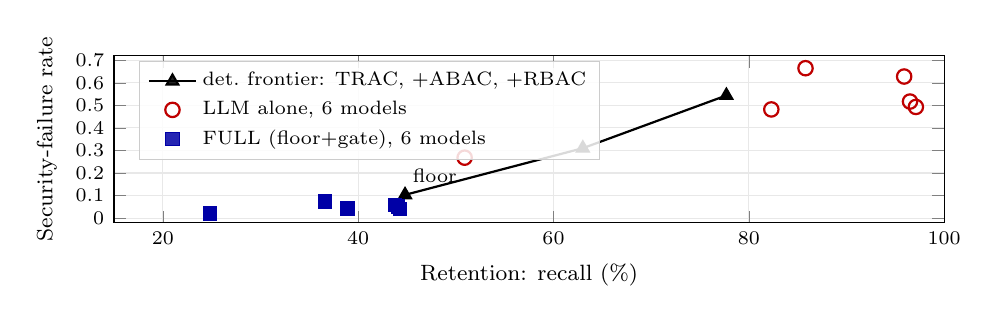
\begin{tikzpicture}
\begin{axis}[
    width=\columnwidth, height=3.7cm,
    xlabel={Retention: recall (\%)}, ylabel={Security-failure rate},
    xmin=15, xmax=100, ymin=-0.02, ymax=0.72,
    xtick={20,40,60,80,100}, ytick={0,0.1,0.2,0.3,0.4,0.5,0.6,0.7},
    grid=major, grid style={gray!18},
    tick label style={font=\scriptsize}, label style={font=\footnotesize},
    legend style={font=\scriptsize, at={(0.03,0.97)}, anchor=north west,
                  cells={anchor=west}, fill=white, fill opacity=0.85,
                  text opacity=1, draw=gray!40},
    legend cell align={left},
]
% Deterministic frontier (bundle-only, model-independent): TRAC-only -> +ABAC -> +RBAC (floor)
\addplot[thick, black, mark=triangle*, mark size=2.4pt]
  coordinates {(77.7,0.544) (63.0,0.310) (44.8,0.103)};
\addlegendentry{det.\ frontier: TRAC, +ABAC, +RBAC}
% LLM alone: 6 models across 3 vendors
\addplot[only marks, mark=o, mark size=2.6pt, red!75!black, thick]
  coordinates {(50.9,0.268) (85.8,0.665) (82.3,0.482) (97.1,0.493) (96.5,0.517) (95.9,0.628)};
\addlegendentry{LLM alone, 6 models}
% FULL = floor + gate: 6 models across 3 vendors
\addplot[only marks, mark=square*, mark size=2.4pt, blue!65!black]
  coordinates {(24.8,0.021) (36.6,0.073) (38.9,0.043) (44.3,0.040) (44.1,0.051) (43.8,0.059)};
\addlegendentry{FULL (floor+gate), 6 models}
\node[font=\scriptsize, anchor=south west] at (axis cs:44.6,0.115) {floor};
\end{axis}
\end{tikzpicture}
\caption{Operating-point map: security-failure rate vs.\ retention (recall, \% of \emph{domain-eligible} requests admitted). The model-independent deterministic frontier (TRAC $\to$ $+$ABAC $\to$ $+$RBAC) is monotone; every LLM-only validator sits well above it at high security-failure \emph{regardless} of retention, while composing each model's verdict behind the floor (FULL) pulls all six models, across three vendors, into a tight low-security-failure cluster ($\leq7.3\%$), none exceeding the $10.3\%$ floor. Retention counts \emph{every} denied domain-eligible request, including \emph{intended} least-privilege denials by RBAC/ABAC; policy-conditioned availability (admissible-only) is higher ($80.7\%$, \S\ref{sec:policy_dependence}). Values: Table~\ref{tab:stack_guarantee}; replay via \texttt{scripts/sweep\_op\_points.py}.}
\Description{Scatter plot of security-failure rate against retention (recall). The deterministic policy frontier descends as TRAC, ABAC, and RBAC are added; LLM-only points sit above it at high security-failure, while full-pipeline points cluster near low security-failure at the secure end.}
\label{fig:operating_sweep}
\end{figure}

The deterministic layers trace a \emph{monotone} frontier---each added layer lowers the security-failure rate ($54\%\!\to\!31\%\!\to\!10\%$) at a retention cost; every LLM-only point sits well above it whatever its retention, while composing the model behind the floor (FULL) collapses all six models across three vendors into a tight low-security-failure cluster ($\leq7.3\%$), none exceeding the $10.3\%$ floor (\S\ref{sec:reversal}).

\textbf{The security/retention trade-off.} The floor's \emph{retention}---recall $0.448$, i.e.\ $44.8\%$ of \emph{domain-eligible} (task-correct \emph{and} domain-authorised) requests admitted---is deliberately conservative, but it \emph{understates} availability. Of the $1{,}091$ denied, $879$ are correct bundles RBAC/ABAC deny because their tools exceed the role's fine-grained grant---the label authorises at the \emph{domain} level while enforcement is at the \emph{tool} level, so these are \emph{intended} least-privilege, not lost availability. Conditioned on genuinely \emph{admissible} work---the $1{,}098$ requests that are task-correct \emph{and} fully authorised---the floor's \textbf{policy-conditioned availability is $80.7\%$} ($886/1098$) at a \textbf{false-block rate of $19.3\%$} ($212/1098$), the latter entirely the leak-free task-relational layer's imperfect domain inference and tunable (\S\ref{sec:policy_dependence}). The low retention is thus a deliberate max-security operating point on a policy-navigable frontier, not a fixed limit.

\subsubsection{Per-Persona Floor}
\label{sec:persona_floor}

The aggregate floor is a mean over six personas whose funnels differ sharply (Table~\ref{tab:persona_floor}); because the deterministic layers condition only on persona, bundle, and inferred domain, this decomposition is model-independent. Narrowly-scoped roles admit very little: Research (L1) retains only $22/1157$ ground-truth bundles after the selection floor and $11$ after validation---RBAC's tight grant leaves few same-domain wrong-tool bundles for the semantic layer to miss. Broad L3 infrastructure roles (DevOps, Gateway, Security) admit far more at every gate---DevOps $632$, Gateway $487$, Security $367$ selection survivors---shifting the discrimination burden onto the leak-free TRAC predicate. This per-role spread under one fixed policy is why an agnostic floor is a \emph{floor}, not a solution: the model gate must equalise it (\S\ref{sec:whole_flow}).

\begin{table}[!t]
\centering
\caption{Per-persona survivor funnels supporting the deterministic-floor analysis (RBAC$\to$ABAC$\to$TRAC; model-independent, $n=6{,}942$). Each cell is the number of requests \emph{still admitted} after that cumulative gate. \emph{Selection}: every task's ground-truth bundle (perfect selection), gated RBAC$\to$ABAC$\to$TRAC. \emph{Validation}: all candidate bundles, with an oracle correctness filter (the \textbf{Oracle} column)---a construction device to isolate the deterministic layers on the valid cohort, \emph{not} part of the floor---rejecting every incorrect bundle, gated RBAC$\to$ABAC$\to$Oracle$\to$TRAC. Narrowly-scoped roles (Research, Finance) admit few; broad L3 roles (DevOps, Gateway, Security) admit many, shifting the burden onto TRAC. Totals give floor precision (security) $0.63$, recall (retention) $0.45$, security-failure $10.3\%$ (policy-conditioned availability $80.7\%$).}
\label{tab:persona_floor}
\footnotesize
\setlength{\tabcolsep}{5pt}
\begin{adjustbox}{max width=\columnwidth}
\begin{tabular}{@{}lccccc@{}}
\toprule
\textbf{Persona} & \textbf{total} & \textbf{RBAC} & \textbf{ABAC} & \textbf{Oracle} & \textbf{TRAC} \\
\midrule
\multicolumn{6}{@{}l}{\textit{Selection --- ground-truth bundles; gates RBAC$\to$ABAC$\to$TRAC}}\\
DevOps \textit{(L3)}   & 1157 &  770 &  770 & --- &  632 \\
Incident \textit{(L2)} & 1157 &  307 &  260 & --- &  231 \\
Finance \textit{(L2)}  & 1157 &  141 &   43 & --- &   41 \\
Research \textit{(L1)} & 1157 &   63 &   63 & --- &   22 \\
Gateway \textit{(L3)}  & 1157 &  628 &  616 & --- &  487 \\
Security \textit{(L3)} & 1157 &  510 &  454 & --- &  367 \\
\textbf{Total}         & 6942 & 2419 & 2206 & --- & 1780 \\
\midrule
\multicolumn{6}{@{}l}{\textit{Validation --- all candidates $+$ oracle reject-all; gates RBAC$\to$ABAC$\to$Oracle$\to$TRAC}}\\
DevOps \textit{(L3)}   & 1157 &  748 &  748 &  384 &  314 \\
Incident \textit{(L2)} & 1157 &  303 &  254 &  129 &  114 \\
Finance \textit{(L2)}  & 1157 &  124 &   37 &   21 &   20 \\
Research \textit{(L1)} & 1157 &   78 &   78 &   30 &   11 \\
Gateway \textit{(L3)}  & 1157 &  639 &  627 &  306 &  242 \\
Security \textit{(L3)} & 1157 &  514 &  462 &  228 &  185 \\
\textbf{Total}         & 6942 & 2406 & 2206 & 1098 &  886 \\
\bottomrule
\end{tabular}
\end{adjustbox}
\end{table}

\subsection{The LLM Alone}
\label{sec:llm_alone}

Removing the deterministic floor and letting the model judge or select unaided shows how a single LLM behaves as a control. We score it at \emph{task} resolution over the $1{,}157$-task corpus (persona-invariant, \S\ref{sec:resolution_gap}) with the correct bundle as the positive class---its intrinsic semantic-judgment quality, independent of any policy.

Table~\ref{tab:llm_pr} reports both modes for all six models: \emph{validation}, where the model judges a candidate bundle and has a scoreable admit/deny verdict (precision, recall, $F_1$, accuracy); and \emph{selection}, where it generates the bundle and is scored on recovery of the task's three gold tools (graded $k/3$ counts, exact-match rate, Jaccard). gpt-3.5-turbo-16k has no selection run---its candidate-catalog prompt exceeds context.

\begin{table}[!t]
\centering
\caption{The LLM alone, both modes, at task resolution ($n=1{,}157$ tasks, persona-invariant; positive class $=$ correct bundle). \emph{Validation} (top): the model judges a candidate bundle---precision, recall, $F_1$, accuracy of its admit/deny verdict. \emph{Selection} (bottom): the model generates the bundle and is scored on recovery of the task's three gold tools ($k/3$ counts over all $1{,}157$ tasks, exact-match rate, mean Jaccard). Recall is high for the 2026 cross-vendor models but precision (security) never exceeds $0.78$; selection is far weaker (best exact-match $9.4\%$). Neither mode is monotone in recency (\S\ref{sec:newer_not_better}). Positive $=$ valid (persona-relative) system scoring of these same runs is \S\ref{sec:resolution_gap}.}
\label{tab:llm_pr}
\footnotesize
\setlength{\tabcolsep}{5pt}
\begin{adjustbox}{max width=\columnwidth}
\begin{tabular}{@{}lcccc@{}}
\toprule
\textbf{Validation --- LLM as judge} & \textbf{P} & \textbf{R} & $\mathbf{F_1}$ & \textbf{Acc} \\
\midrule
gpt-3.5-turbo-16k \textit{(OpenAI '23)}    & 0.705 & 0.815 & 0.756 & 0.736 \\
gpt-4o \textit{(OpenAI '24)}               & 0.740 & 0.497 & 0.595 & 0.661 \\
gpt-5.4 \textit{(OpenAI '26)}              & 0.583 & 0.839 & 0.688 & 0.620 \\
claude-opus-4.8 \textit{(Anthropic '26)}   & 0.772 & \textbf{0.971} & \textbf{0.860} & \textbf{0.842} \\
claude-sonnet-4.6 \textit{(Anthropic '26)} & 0.748 & 0.964 & 0.842 & 0.819 \\
gemini-2.5-pro \textit{(Google '26)}       & 0.666 & 0.962 & 0.787 & 0.740 \\
\bottomrule
\end{tabular}
\end{adjustbox}

\vspace{4pt}
\begin{adjustbox}{max width=\columnwidth}
\begin{tabular}{@{}lcccccc@{}}
\toprule
\textbf{Selection --- LLM as generator} & \textbf{3/3} & \textbf{2/3} & \textbf{1/3} & \textbf{0/3} & \textbf{Exact} & \textbf{Jacc.} \\
\midrule
gpt-3.5-turbo-16k \textit{('23)} & \multicolumn{6}{c}{\textit{n/a --- catalog prompt $>$ context}} \\
gpt-4o \textit{('24)}            &  52 & 189 & 304 & 612 & 4.5\% & 0.179 \\
gpt-5.4 \textit{('26)}           &  66 & 206 & 292 & 593 & 5.7\% & 0.197 \\
claude-opus-4.8 \textit{('26)}   & 109 & 228 & 260 & 560 & \textbf{9.4\%} & \textbf{0.238} \\
claude-sonnet-4.6 \textit{('26)} &  93 & 221 & 290 & 553 & 8.0\% & 0.226 \\
gemini-2.5-pro \textit{('26)}    &  28 & 104 & 274 & 751 & 2.4\% & 0.117 \\
\bottomrule
\end{tabular}
\end{adjustbox}
\end{table}

\subsubsection{Task Resolution vs.\ Authorisation Resolution}
\label{sec:resolution_gap}

The verdict is \emph{persona-invariant}: for every one of the $1{,}157$ tasks the model returns an \emph{identical} admit/deny for the candidate bundle whichever of the six personas issued it ($1157/1157$ tasks, every panel model). The $6{,}942$-row system view is therefore $1{,}157$ semantic judgments replicated six-fold---the model decides at \emph{task} resolution, blind to the requester. Authorisation, however, is persona-relative: on each of the $579$ task-\emph{correct} bundles legitimacy depends on the role---valid for some personas, a least-privilege \emph{violation} for others (\S\ref{sec:dataset})---yet the persona-blind model admits the correct bundle for all six, passing the violations silently. Scored as an \emph{authorisation} control under the system convention (positive $=$ valid, \S\ref{sec:conventions}), the unaided model's security-failure rate spans $26.8$--$66.5\%$ across the panel (gpt-4o best at $26.8\%$, gpt-5.4 worst at $66.5\%$)---the mechanistic form of our thesis (\S\ref{sec:motivation}): \emph{semantic correctness is not authorisation correctness}. RBAC exists to supply exactly the persona resolution the model structurally lacks (\S\ref{sec:reversal}).

\subsubsection{Independent Replication of ASTRA's LLM-ResM Benchmark}
\label{sec:astra_replication}

At task resolution (positive $=$ correct bundle, $n=1{,}157$, matching ASTRA's permissivity setting), our gpt-4o reaches $F_1=0.595$ vs.\ ASTRA's published $0.67$---a $0.075$ gap under a strictly harder protocol (ASTRA AND-aggregates three per-tool verdicts, inflating precision; we use one per-bundle call), so our number is the expected lower bound. The precision--recall signature replicates: high precision ($0.740$ vs.\ $0.81$), low recall ($0.497$ vs.\ $0.57$), under-scoping dominant; the two other OpenAI generations bracket gpt-4o ($0.756$, $0.688$). A reproduction of ASTRA's under-scoping finding, not a refutation.

\subsubsection{Non-Monotone LLM-Only Behaviour with Model Recency}
\label{sec:newer_not_better}

A clean side-effect of the three OpenAI generations: LLM-only safety is \emph{non-monotone} in recency (the ordering differs by metric). By semantic $F_1$ (positive $=$ correct), gpt-3.5-turbo-16k (2023, $0.756$) beats gpt-4o (2024, $0.595$) and gpt-5.4 (2026, $0.688$); as an authorisation control (security-failure rate), gpt-4o is strongest ($26.8\%$) yet the 2026 gpt-5.4 is the \emph{most} permissive ($66.5\%$ vs.\ $26.8\%$). We cannot causally attribute this without a controlled fine-tune, but the lesson holds across vendors---every $2026$ model is a \emph{more} permissive validator than the 2023 one (\S\ref{sec:cross_vendor})---so \emph{a single-LLM validator cannot be assumed to improve as base models advance}.

\subsection{The Whole Flow: Composition and Recovery}
\label{sec:whole_flow}

Composing the two---the model's verdict \emph{behind} the deterministic floor---is the deployed system. We read the composition three ways, each results-first: a cross-vendor validation panel showing the floor bounds every model's security-failure rate whatever its solo behaviour (\S\ref{sec:stack_guarantee}); a per-model survivor funnel for claude-opus-4.8 (the highest-retention composition) that shows \emph{where} each layer catches (\S\ref{sec:whole_flow_funnels}); and a model-independent layer ablation isolating each layer's marginal contribution (\S\ref{sec:reversal}).

\subsubsection{Cross-Vendor Validation: The Floor Bounds Security Failure}
\label{sec:stack_guarantee}
\label{sec:cross_vendor}

PALADIN is deployed as FULL $=$ the model's own verdict \emph{behind} the deterministic floor; it complements the LLM rather than replacing it. Table~\ref{tab:stack_guarantee} reads that composition across six models spanning three vendors, each judging every candidate bundle \emph{blind} to the ground-truth label with the \emph{same} \texttt{ValidationService} rubric (verdicts frozen before scoring and released).

\begin{table}[!t]
\centering
\caption{Cross-vendor validation composition (system convention, positive $=$ valid, $n=6{,}942$ per model). Six models, three vendors, each judging blind with the \emph{same} rubric. \textbf{LLM alone} $=$ the verdict with no policy; \textbf{FULL} $=$ the same verdict behind the model-independent floor (listed once). $P_{\text{sec}}$ is precision (security), $R_{\text{ret}}$ recall (domain-eligible retention), sec-fail the fraction of not-valid admitted. Every model is permissive alone (sec-fail $0.27$--$0.67$) yet the floor bounds all six to $\leq7.3\%$ once composed; none exceeds the $10.3\%$ floor. Composition trades retention for security by model: the strictest judge (gpt-4o) reaches sec-fail $0.021$ at $R_{\text{ret}}\,0.248$, while claude-opus-4.8 holds $R_{\text{ret}}\,0.443$ at sec-fail $0.040$. Task-level bootstrap CIs ship with the artefact.}
\label{tab:stack_guarantee}
\footnotesize
\setlength{\tabcolsep}{6pt}
\begin{adjustbox}{max width=\columnwidth}
\begin{tabular}{@{}lcccc@{}}
\toprule
 & \textbf{alone} & \multicolumn{3}{c}{\textbf{FULL (floor$+$gate)}} \\
\cmidrule(lr){2-2}\cmidrule(lr){3-5}
\textbf{Model (vendor, year)} & \textbf{sec-fail} & $\mathbf{P_{\text{sec}}}$ & $\mathbf{R_{\text{ret}}}$ & \textbf{sec-fail} \\
\midrule
\multicolumn{5}{@{}l}{\textbf{Deterministic floor} \textit{(model-independent)}: $P_{\text{sec}}\,0.634$, $R_{\text{ret}}\,0.448$, sec-fail $0.103$}\\
\midrule
gpt-3.5-turbo-16k \textit{(OpenAI '23)}    & 0.482 & 0.780 & 0.389 & 0.043 \\
gpt-4o \textit{(OpenAI '24)}               & 0.268 & 0.824 & 0.248 & \textbf{0.021} \\
gpt-5.4 \textit{(OpenAI '26)}              & 0.665 & 0.665 & 0.366 & 0.073 \\
\addlinespace[2pt]
claude-opus-4.8 \textit{(Anthropic '26)}   & 0.493 & 0.816 & \textbf{0.443} & 0.040 \\
claude-sonnet-4.6 \textit{(Anthropic '26)} & 0.517 & 0.775 & 0.441 & 0.051 \\
gemini-2.5-pro \textit{(Google '26)}       & 0.628 & 0.747 & 0.438 & 0.059 \\
\bottomrule
\end{tabular}
\end{adjustbox}
\end{table}

Alone, each model is an unreliable control: security-failure spans $26.8\%$ (gpt-4o) to $66.5\%$ (gpt-5.4), non-OpenAI models interleaved throughout, no ordering by vendor or recency. Behind the floor, the same verdict is bounded to security-failure $\leq7.3\%$ for all six, none exceeding the $10.3\%$ floor---because FULL $=$ floor $\wedge$ verdict is a conjunction that can only \emph{add} denials, so a capable judge (gpt-4o) sharpens security-failure to $2.1\%$ while even a permissive one cannot lift FULL above the floor (P1, \S\ref{sec:composition}). The composition is \emph{leak-free}: the domain driving coverage is inferred from task text by BM25 over the public MCP catalog (\S\ref{sec:domain_inference}), so the floor sits at $10.3\%$ rather than zero---the irreducible semantic floor the verdict, not the policy, must close.

\textbf{Security vs.\ retention is now a per-model choice.} Composition sharpens security for every model, but at a recall (retention) cost that differs sharply: gpt-4o drives security-failure to $2.1\%$ yet admits only $24.8\%$ of domain-eligible work, whereas claude-opus-4.8 holds retention at $44.3\%$ for a near-identical $4.0\%$ security-failure. opus is thus the highest-retention composition on the panel and gpt-4o the strictest; we trace opus as a survivor funnel next (\S\ref{sec:whole_flow_funnels}).

\paragraph{Operating point.} The floor profile comes from the released policy---the \path{capability_coverage} domain floor, the \path{tool_relevance} BM25 cutoff ($<\!1.0$), and the corroborated-coverage rescue bar ($\geq\!4.0$), all editable in \path{policies/trac_rules.yaml} and fixed \emph{ex ante}; \S\ref{sec:corroborated} gives the Pareto refinement that sets it.

\subsubsection{Whole-Flow Funnel for the Highest-Retention Model}
\label{sec:whole_flow_funnels}

Table~\ref{tab:flow_opus} traces claude-opus-4.8 through the whole flow as a survivor funnel: the count still admitted after each cumulative gate, restricted to the requests that stress the system. The two blocks use \emph{different} incorrect cohorts by construction. \emph{Validation} gates the $578$ wrong$/$null \emph{candidate} bundles per persona---the bundles the model is asked to judge. \emph{Selection} gates the $1{,}048$ tasks per persona where opus's \emph{own} pick recovered fewer than $3/3$ ground-truth tools (the $2/3\!+\!1/3\!+\!0/3$ buckets of \S\ref{sec:llm_alone}), since in selection the model \emph{is} the requester and the honest incorrect subset is the bundles it mis-selects. The final column is the residual security failures.

\begin{table}[!t]
\centering
\caption{claude-opus-4.8 whole-flow survivor funnels (the highest-retention model). Each cell is the number \emph{still admitted} after that cumulative gate. \emph{Validation}: the $578$ wrong$/$null \emph{candidate} bundles per persona ($n=3{,}468$), gated RBAC$\to$ABAC$\to$LLM verdict$\to$TRAC; $198$ survive. \emph{Selection}: the $1{,}048$ tasks per persona where opus's \emph{own} pick recovered $<3/3$ gold tools ($n=6{,}288$; the $2/3\!+\!1/3\!+\!0/3$ buckets of \S\ref{sec:llm_alone}), gated RBAC$\to$ABAC$\to$TRAC; $1{,}805$ survive. In validation, RBAC and ABAC condition only on persona and bundle, so their columns are model-independent; ABAC removes little beyond RBAC ($1108$ vs.\ $1200$), the backstop pattern of \S\ref{sec:reversal}.}
\label{tab:flow_opus}
\footnotesize
\setlength{\tabcolsep}{5pt}
\begin{adjustbox}{max width=\columnwidth}
\begin{tabular}{@{}lccccc@{}}
\toprule
\textbf{Persona} & \textbf{total} & \textbf{RBAC} & \textbf{ABAC} & \textbf{LLM} & \textbf{TRAC} \\
\midrule
\multicolumn{6}{@{}l}{\textit{Validation --- incorrect tasks; gates RBAC$\to$ABAC$\to$LLM$\to$TRAC}}\\
DevOps \textit{(L3)}   &  578 &  364 &  364 &   98 &   55 \\
Incident \textit{(L2)} &  578 &  150 &  125 &   45 &   26 \\
Finance \textit{(L2)}  &  578 &   52 &   16 &    3 &    3 \\
Research \textit{(L1)} &  578 &   48 &   48 &   23 &    7 \\
Gateway \textit{(L3)}  &  578 &  327 &  321 &  109 &   56 \\
Security \textit{(L3)} &  578 &  259 &  234 &   94 &   51 \\
\textbf{Total}         & 3468 & 1200 & 1108 &  372 &  198 \\
\midrule
\multicolumn{6}{@{}l}{\textit{Selection --- opus's own wrong picks ($<3/3$ recovered; $1{,}048$/persona); gates RBAC$\to$ABAC$\to$TRAC}}\\
DevOps \textit{(L3)}   & 1048 &  689 &  689 &  --- &  562 \\
Incident \textit{(L2)} & 1048 &  333 &  287 &  --- &  245 \\
Finance \textit{(L2)}  & 1048 &  146 &   89 &  --- &   78 \\
Research \textit{(L1)} & 1048 &   60 &   60 &  --- &   21 \\
Gateway \textit{(L3)}  & 1048 &  666 &  622 &  --- &  480 \\
Security \textit{(L3)} & 1048 &  586 &  524 &  --- &  419 \\
\textbf{Total}         & 6288 & 2480 & 2271 &  --- & 1805 \\
\bottomrule
\end{tabular}
\end{adjustbox}
\end{table}

In validation, RBAC and ABAC condition only on persona and bundle, so they are model-independent ($1{,}200$ then $1{,}108$ survivors); ABAC's marginal is small ($92$ caught) because RBAC already denies most of what ABAC would---the backstop pattern quantified next (\S\ref{sec:reversal}). opus's own verdict then admits $372$ of the $1{,}108$, and TRAC catches a further $174$ ($372\!\to\!198$) incorrect tasks the verdict let through---the task-relational layer working behind the model. The security$/$retention trade a stricter or more permissive judge would make behind this same floor is the per-model panel of Table~\ref{tab:stack_guarantee}.

\paragraph{Selection.}
\label{sec:selection_flow}
When the model \emph{generates} the bundle there is no verdict gate, yet the same RBAC$\to$ABAC$\to$TRAC floor still removes $4{,}483/6{,}288$ of the bundles opus mis-selects (the $1{,}048$ tasks per persona where it recovered $<3/3$ gold tools), so the deterministic stack recovers generation failures as well as verdict failures without re-tuning.

\subsubsection{Which Layers Are Load-Bearing}
\label{sec:reversal}

\begin{table}[!t]
\centering
\caption{Full-factorial layer ablation on the deterministic stack (validation, $n=6{,}942$; model-independent). $R_{\text{ret}}$ is recall (domain-eligible retention); sec-fail is the security-failure rate (lower is safer; numerically identical to the earlier security-failure metric). \emph{Every} ablation is worse on security than the full stack: conventional access control alone (RBAC$+$ABAC, no task-relational layer) leaves sec-fail at $0.223$---more than double the full stack's $0.103$, the operating point of any conventional AC method without the predicate (\S\ref{sec:access_control}). The \textbf{drop-one} column gives the omitted layer's order-independent marginal (sec-fail of the full stack minus this row). Frontier in Fig.~\ref{fig:ablation_frontier}; per-model composition in Table~\ref{tab:stack_guarantee}.}
\label{tab:factorial_ablation}
\footnotesize
\setlength{\tabcolsep}{6pt}
\begin{adjustbox}{max width=\columnwidth}
\begin{tabular}{@{}lccc@{}}
\toprule
\textbf{Configuration} & $\mathbf{R_{\text{ret}}}$ & \textbf{sec-fail} & \textbf{drop-one} \\
\midrule
No policy (all open)             & 1.000 & 1.000 & --- \\
\addlinespace[2pt]
RBAC only                        & 0.610 & 0.242 & --- \\
TRAC only                        & 0.777 & 0.544 & --- \\
ABAC only                        & 0.810 & 0.610 & --- \\
\addlinespace[2pt]
RBAC$+$TRAC \textit{($-$ABAC)}   & 0.496 & 0.112 & ABAC $-0.9$pp \\
RBAC$+$ABAC \textit{($-$TRAC)}   & 0.555 & 0.223 & TRAC $-12.0$pp \\
ABAC$+$TRAC \textit{($-$RBAC)}   & 0.630 & 0.310 & RBAC $-20.7$pp \\
\midrule
\textbf{RBAC\,$\wedge$\,ABAC\,$\wedge$\,TRAC (full)} & 0.448 & \textbf{0.103} & --- \\
\bottomrule
\end{tabular}
\end{adjustbox}
\end{table}

\begin{figure}[!t]
\centering
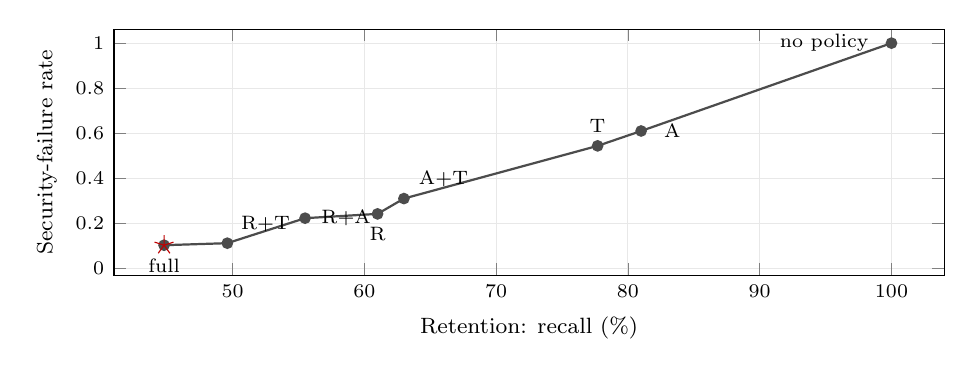
\begin{tikzpicture}
\begin{axis}[
    width=\columnwidth, height=4.7cm,
    xlabel={Retention: recall (\%)}, ylabel={Security-failure rate},
    xmin=41, xmax=104, ymin=-0.03, ymax=1.06,
    xtick={50,60,70,80,90,100}, ytick={0,0.2,0.4,0.6,0.8,1.0},
    grid=major, grid style={gray!18},
    tick label style={font=\scriptsize}, label style={font=\footnotesize},
]
% Deterministic ablation frontier: all eight layer subsets, monotone in admission.
\addplot[thick, black!70, mark=*, mark size=1.7pt]
  coordinates {(44.8,0.103) (49.6,0.112) (55.5,0.223) (61.0,0.242)
               (63.0,0.310) (77.7,0.544) (81.0,0.610) (100.0,1.000)};
% Full stack highlighted.
\addplot[only marks, mark=star, mark size=3.6pt, red!75!black]
  coordinates {(44.8,0.103)};
\node[font=\scriptsize, anchor=north]      at (axis cs:44.8,0.086) {full};
\node[font=\scriptsize, anchor=south west] at (axis cs:49.9,0.118) {R$+$T};
\node[font=\scriptsize, anchor=west]       at (axis cs:56.0,0.223) {R$+$A};
\node[font=\scriptsize, anchor=north]      at (axis cs:61.0,0.228) {R};
\node[font=\scriptsize, anchor=south west] at (axis cs:63.4,0.320) {A$+$T};
\node[font=\scriptsize, anchor=south]      at (axis cs:77.7,0.560) {T};
\node[font=\scriptsize, anchor=west]       at (axis cs:82.0,0.610) {A};
\node[font=\scriptsize, anchor=east]       at (axis cs:99.0,1.000) {no policy};
\end{axis}
\end{tikzpicture}
\caption{Ablation operating points: security-failure rate vs.\ retention (recall) for all eight subsets of the deterministic stack (validation; model-independent; R\,$=$\,RBAC, A\,$=$\,ABAC, T\,$=$\,TRAC). Adding a layer lowers the security-failure rate at a retention cost, tracing a monotone frontier with the full stack (star) at the secure end (sec-fail\,$0.103$). Most of the retention gap is RBAC/ABAC least-privilege denial of correct bundles that exceed the role's fine-grained grant---\emph{intended} enforcement, not lost availability (\S\ref{sec:operating_sweep}). Values: Table~\ref{tab:factorial_ablation}.}
\Description{Scatter plot with a connecting line showing security-failure rate against retention (recall) for all eight layer subsets. As layers are added, retention decreases and the security-failure rate decreases monotonically, with the full RBAC-ABAC-TRAC stack at the low-retention, low-security-failure secure end and the no-policy baseline at full retention and security-failure one.}
\label{fig:ablation_frontier}
\end{figure}

Table~\ref{tab:factorial_ablation} scores all eight subsets of the deterministic stack (validation; deterministic, hence model-independent): \emph{every} ablation is strictly worse on security than the full stack, and conventional access control alone---RBAC$+$ABAC with no task-relational layer---leaves security-failure at $0.223$, more than double the full stack's $0.103$ (frontier in Fig.~\ref{fig:ablation_frontier}). The honest per-layer measure is the order-independent \emph{drop-one} marginal---the security-failure of the full stack vs.\ the stack with exactly that one layer removed. RBAC ($-20.7$pp, $95\%$ CI $[-22.6,-19.0]$) and \textbf{TRAC ($-12.0$pp, $[-13.5,-10.6]$)} are each individually load-bearing---both CIs exclude $0$---whereas \textbf{ABAC's drop-one marginal is only $-0.9$pp} ($[-1.3,-0.6]$), because ABAC and RBAC \emph{overlap}: most attribute violations ABAC would catch are already caught by RBAC. ABAC is therefore a \emph{backstop}: near-redundant given RBAC on this benchmark, but load-bearing when RBAC is absent (removing ABAC once RBAC is already gone costs a further $23.4$pp). This same overlap surfaces concretely in the funnels of \S\ref{sec:whole_flow_funnels}, where ABAC removes only $92$ of $1{,}200$ RBAC survivors.

Two readings follow. TRAC's isolated $-12.0$pp is direct evidence the task-relational axis catches violations conventional RBAC$+$ABAC cannot---measured, not asserted. And the gap between ABAC's first-firing share and its drop-one marginal instances the attribution pitfall of \S\ref{sec:attribution_paradox}: a layer can look essential under one lens and near-redundant under another, so both must be reported---guidance not ``never drop a layer'' but ``RBAC and TRAC are individually load-bearing; ABAC hedges RBAC.'' This also corrects the earlier oracle-aided policy, in which an alignment score did most of the validation work and RBAC/ABAC were near-redundant; removing the oracle redistributes the security load onto identity and the task-relational predicate---exactly where a zero-trust deployment can audit it.

\textbf{Is the load-bearing pattern a label artefact?} Two decouplings say no. Re-authoring RBAC \emph{independently} of the label (coarse job-function roles that \emph{over-provision} relative to the fine-grained allow-list) shrinks RBAC's drop-one marginal ($-20.7\!\to\!-11.3$pp), but the slack redistributes onto TRAC ($-12.0\!\to\!-21.5$pp) and ABAC ($-0.9\!\to\!-9.1$pp) and the floor degrades gracefully (security-failure $10.3\!\to\!19.7\%$) while admitting strictly more legitimate work---no single layer's exact tuning is load-bearing. Decoupling the \emph{label} itself from all policy (legitimacy from ASTRA's \texttt{match\_tag} alone, dropping the persona--domain criterion) makes \textbf{TRAC's marginal \emph{rise} to $-17.2$pp $[-19.1,-15.5]$, the largest of the three} (paired task-level bootstrap $95\%$ CI clear of $0$; RBAC falls to $-14.6$pp $[-16.5,-12.7]$): under a label no policy artefact authored, the task-relational predicate is the \emph{most} load-bearing layer---the opposite of a circularity artefact.

\textbf{The enforcing surface is not only lexical.} Two TRAC rules reason about \emph{action semantics}: \texttt{action\_coherence} (read-intent task, mutating tools) and \texttt{write\_safety} (destructive op without a preceding read). Making \texttt{action\_coherence} enforcing catches $39$ same-domain violations the BM25 predicates and RBAC$+$ABAC all miss, at precision $0.62$ ($1.69\times$ the approved base rate), lowering security-failure $10.3\!\to\!9.5\%$ at $24$ new legitimate blocks---structural coherence beyond BM25. (\texttt{write\_safety} is weaker, precision $0.31$, so advisory.)

\subsubsection{Best-Effort Adversarial Rule Design}
\label{sec:llm_authored}

The sharpest challenge to the load-bearing claim is that our particular RBAC and ABAC might simply be under-tuned: perhaps a \emph{better} conventional policy---one we failed to write---would reach the floor without any task-relational layer, rendering TRAC redundant. We test this adversarially by outsourcing the rule design to the strongest available policy authors and asking whether any of them closes the gap. Three frontier LLMs---\texttt{claude-opus-4.8} (Anthropic), \texttt{gpt-5.4} (OpenAI), and \texttt{gemini-3.1-pro} (Google), one per vendor---each \emph{independently} authored a complete RBAC$+$ABAC policy from a leak-free brief: the six persona attributes (\S\ref{sec:policy_details}), the nine domains with their resource attributes, a per-domain tool taxonomy (read / benign-write / privileged-write / destructive-write counts), both rule grammars, and the stated objective---deny \texttt{wrong} and \texttt{null} bundles while admitting correct in-scope work. Crucially the brief withholds every artefact from which the answer could be copied: no persona--domain pairings, no per-row labels, and none of our shipped rules. Each authored policy is then evaluated through the \emph{identical} stack with TRAC frozen at production (\S\ref{sec:trac}); the deterministic floor is model-independent, so one validation replay per policy recovers the full confusion matrix. An audit confirmed independence---no author reconstructed the released grants (at most one persona coincided incidentally)---and every policy stayed within the least-privilege objective, with no degenerate blanket-deny rule that would trade all availability for a low floor.

\begin{table}[!t]
\centering
\caption{Best-effort adversarial rule design: three frontier LLMs (one per vendor) each \emph{independently} author a complete RBAC$+$ABAC policy from a leak-free brief (no labels, pairings, or shipped rules); TRAC is frozen at production. Validation, $n=6{,}942$, model-independent; the domain-eligible ($1{,}977$) and not-valid ($4{,}965$) sets are constant across policies, so every row is comparable. sec-fail is the security-failure rate (lower safer); $R_{\text{ret}}$ is retention (recall); \emph{no TRAC} is the same policy's sec-fail with the task-relational layer removed (RBAC$+$ABAC only); \emph{drop-one} is TRAC's order-independent marginal on that policy. \emph{No} authored conventional stack (no-TRAC column) reaches the full stack's $0.103$ floor, and TRAC's marginal is strictly negative---load-bearing---on every one. Rows ordered by permissiveness; PALADIN production shown for reference.}
\label{tab:llm_authored}
\footnotesize
\setlength{\tabcolsep}{5pt}
\begin{adjustbox}{max width=\columnwidth}
\begin{tabular}{@{}lcccc@{}}
\toprule
\textbf{Policy author} & $\mathbf{R_{\text{ret}}}$ & \textbf{sec-fail} & \textbf{no TRAC} & \textbf{TRAC drop-one} \\
\midrule
Opus 4.8 \textit{(strictest)}  & 0.340 & 0.095 & 0.190 & $-9.5$pp \\
GPT-5.4                        & 0.434 & 0.111 & 0.252 & $-14.1$pp \\
Gemini 3.1 Pro \textit{(most permissive)} & 0.576 & 0.158 & 0.347 & $-18.9$pp \\
\midrule
\textbf{PALADIN production}    & 0.448 & \textbf{0.103} & 0.223 & $-12.0$pp \\
\bottomrule
\end{tabular}
\end{adjustbox}
\end{table}

Table~\ref{tab:llm_authored} reports the outcome, and it is decisive on two fronts. \textbf{No authored conventional stack reaches the floor.} The most secure RBAC$+$ABAC policy---Opus 4.8, the strictest author---leaves security-failure at $0.190$ \emph{without} the task-relational layer, still $1.85\times$ the full stack's $0.103$, and buys even that only by collapsing retention to $0.389$. No authored policy---whether its full stack or its no-TRAC variant---attains both $R_{\text{ret}}\!\geq\!0.448$ and sec-fail $\leq\!0.103$; PALADIN's full stack \emph{Pareto-dominates} the best conventional alternative on \emph{both} axes at once. \textbf{TRAC stays load-bearing on every policy.} Its drop-one marginal is strictly negative for all three authors ($-9.5$ to $-18.9$pp) and \emph{grows monotonically} with the policy's permissiveness: the more legitimate work a conventional policy preserves, the more same-domain \texttt{wrong} bundles it necessarily admits---structurally TRAC's to catch (\S\ref{sec:rule_rationale}). Averaged over the panel, TRAC removes $14.2$pp of the $26.3$pp mean conventional-stack security-failure---more than half. Handed the best rules three frontier models can write, conventional access control still cannot close the task-relational gap; this is the strongest form of the label-independence argument above, with the policy authored by an adversary who never saw the labels.


\subsection{In-Depth Analysis}
\label{sec:indepth}

Four analyses probe the result's robustness: why first-firing attribution misranks the layers, how corroborated coverage recovers mis-routed legitimate bundles, why the guarantee is a property of the \emph{policy} rather than our engine (verified OPA/Rego parity), and the dataset ceiling that bounds selection exact-match.

\subsubsection{The Attribution Paradox}
\label{sec:per_domain}
\label{sec:attribution_paradox}

Marginal necessity and first-firing attribution disagree sharply. Attributing every floor denial to the first layer that fires under short-circuit order (RBAC$\to$ABAC$\to$TRAC), RBAC claims $82\%$ of denials, TRAC $15\%$, and ABAC only $4\%$. Yet the marginal picture (\S\ref{sec:reversal}) is the opposite: ABAC, which first-fires on a mere $4\%$ of denials, carries the largest \emph{successive} marginal ($-23.4$pp---removing ABAC once RBAC is already absent), even though its order-independent \emph{drop-one} marginal is only $-0.9$pp. The reason is pipeline order---most rows ABAC would catch are intercepted earlier by RBAC, so ABAC's unique value is invisible to a denial-source chart and surfaces only when RBAC is removed. First-firing attribution, common in the agent-safety literature, therefore systematically misranks layers; both attribution and the marginal security-failure change must be reported.

\subsubsection{Corroborated Coverage}
\label{sec:corroborated}

The leak-free domain classifier (\S\ref{sec:domain_inference}) is intentionally imperfect: a business-phrased task can route to a lexically-similar but wrong MCP, so \texttt{capability\_coverage} occasionally denies a correct, in-domain bundle. \emph{Corroborated coverage} reverses such a denial when an \emph{independent} signal---the mean BM25 relevance of the selected tools to the task---is high ($\geq\!4.0$): a legitimate, domain-mis-routed bundle still has tools that lexically match the task, whereas a genuinely wrong-domain bundle does not. Over the model-independent validation profile, enabling the rescue cuts TRAC's unique over-denials of legitimate work from $233$ to $212$, at a cost of $+0.08$pp security-failure and four lost catches---a small Pareto refinement (the sweep knee is $4.0$) that reintroduces no oracle.

\subsubsection{Substrate Portability: Verified OPA/Rego Parity}
\label{sec:substrate_portability}

The guarantee is a property of the \emph{policy}, not our particular engine. PALADIN's RBAC, ABAC, and TRAC layers are authored as \emph{rules-as-data}: the same YAML documents (\texttt{policies/\{rbac,abac\_rules,trac\_rules\}.yaml}) are evaluated both by our reference Python engine and, \emph{unchanged}, by generic Rego policies on a standard Open Policy Agent runtime (OPA v1.18.0). Editing a rule updates both; no code is generated or hand-synced. We verify decision equivalence with the real \texttt{opa} binary: across $120$ RBAC, $120$ ABAC, and $100$ unique-bundle TRAC evaluations, OPA reproduces \emph{every} ALLOW/DENY decision and every advisory of the reference engine---zero mismatches. Parity holds by construction (both evaluate the identical rule data under the same operator semantics) and is confirmed empirically; the same policies also serve from a live \texttt{opa run --server} instance queried over OPA's REST Data API. The portable boundary is the rule-evaluation layer (S3/S4/S6, \S\ref{sec:framework}); the fact transformer (S5---BM25 domain inference and VerbNet action classification) runs once upstream and supplies both engines the same typed predicates. This is a \emph{deployability} result (\S\ref{sec:trac}): the engine is a commodity, so the task-relational policy is enforceable on standard infrastructure---the artefact is the policy and its predicate, not a new runtime. Benchmarking the \emph{performance} cost of the OPA substrate is the remaining follow-up (\S\ref{sec:future_work}).

\subsubsection{Dataset Ceiling and Post-Hoc Enforcement}
\label{sec:ceiling}

Selection exact-match is intrinsically low (best-in-panel $9.4\%$, \S\ref{sec:llm_alone}): tool-naming pedantry over $194$ non-standardised identifiers, multiple defensible bundles scored against one gold, cross-persona ambiguity, and a brittle all-or-nothing match cap it independently of model capability. Conservatively the practical ceiling is $30$--$40\%$; Jaccard is the less-misleading signal.

\textbf{Post-hoc enforcement.} In selection mode the deterministic stack does not alter the LLM's selections: tool exact-match and Jaccard are recorded per row \emph{before} policy gating, so the policy-gate security-failure differences are purely policy-attributable---PALADIN is a true post-hoc enforcement layer.

%==============================================================================
% SECTION 9: DISCUSSION
%==============================================================================
\FloatBarrier
\section{Discussion}
\label{sec:discussion}

\subsection{Operating Point, Policy Dependence, and Generalisability}
\label{sec:deployment_envelope}
\label{sec:policy_dependence}

The floor's \emph{retention} shortfall has two distinct sources (\S\ref{sec:operating_sweep}). Of the $1{,}091$ denied domain-eligible requests (recall $0.448$ on $1{,}977$), least-privilege enforcement accounts for most: $879$ are correct bundles RBAC/ABAC deny because their tools exceed the role's fine-grained grant---the label authorises at the \emph{domain} level while enforcement is at the \emph{tool} level---\emph{intended} least-privilege, not lost availability. The remaining $212$ are the genuine availability cost---a \emph{false-block rate} of $19.3\%$ on the $1{,}098$ admissible requests (policy-conditioned availability $80.7\%$)---from the two BM25 predicates (\path{capability_coverage}, $160$; \path{tool_relevance}, $52$), of which an \emph{oracle} domain recovers most ($\sim\!5$pp router error, $\sim\!14$pp genuine lexical sparsity, recoverable with a stronger retriever). Nor is the floor fixed: three knobs in \texttt{policies/trac\_rules.yaml} (the \texttt{capability\_coverage} floor, the \texttt{tool\_relevance} cutoff, the rescue bar) and the choice of enforcing layers navigate the frontier (Fig.~\ref{fig:operating_sweep})---TRAC \emph{advisory} at security-failure $22.3\%$, an over-provisioned RBAC (\S\ref{sec:reversal}) at $19.7\%$---so we recommend advisory-TRAC as an availability-balanced default and the full floor where security is paramount (\S\ref{sec:future_work}).

\textbf{Generalisation across tool catalogs.} With one fixed operating point (no per-domain tuning), across ASTRA's eight MCP domains (distinct tool catalogs) the model-independent floor's security-failure rate spans $0$--$21\%$ by domain (\texttt{wikipedia}, a $10$-tool catalog, the outlier)---not overfit to one distribution. Worst-group holds: in \emph{every} catalog the floor's security-failure lies below \emph{every} OpenAI generation's LLM-alone security-failure---per-catalog, not aggregate. So the fixed thresholds are robust \emph{across catalogs within} ASTRA's construction; certifying the signal \emph{beyond} it needs an independently-labelled or second corpus (\S\ref{sec:future_work}).

The guarantee is conditional on the authored policy but bounded: removing any denial rule cannot decrease the security-failure rate (short-circuit), so the per-layer marginals (\S\ref{sec:reversal}) upper-bound the damage from disabling a rule family.

\subsection{The Floor's Adversarial Limit, Quantified}
\label{sec:adversarial}
Our threat model (\S\ref{sec:threat_model}) assumes trusted task provenance---the operator authors the task; the agent proposes only the \emph{bundle}---but we stress-test its violation, which few enforcement papers do. Giving an adversary the task text and appending the bundle's \emph{own} tool names and descriptions (naive prompt-injection-style padding) collapses TRAC's catch on the $578$ bundles it targets from $57.1\%$ to $0.0\%$. Is this specific to the lexical BM25 predicates? We re-instantiate both enforcing predicates with a deterministic local semantic embedding (model2vec, no API): it catches \emph{more} clean ($57.1\!\to\!70.9\%$) yet is \emph{equally} defeated by padding ($70.9\!\to\!4.8\%$). The attack poisons the task text itself, so \emph{no} predicate over that text---lexical or semantic---resists it: the evasion is a property of \emph{untrusted task provenance}, and the control is input integrity (the composed prompt-injection layer, \S\ref{sec:threat_model}), not a stronger relevance function. Within the semi-honest model the guarantee holds; the embedding's higher clean-case catch is an option for deployments willing to trade determinism for a model dependency.

\subsection{Limitations and Threats to Validity}
\label{sec:limitations}

Table~\ref{tab:threats} summarises the dominant threats to validity---internal, external, construct, and statistical---each with its mitigation and a pointer to the relevant section or released artefact.

\begin{table}[!t]
\centering
\caption{Threats to validity at a glance. Mitigations link back to the indicated section or released artefact.}
\label{tab:threats}
\scriptsize
\setlength{\tabcolsep}{3pt}
\begin{tabularx}{\columnwidth}{@{}>{\raggedright\arraybackslash}p{1.8cm}>{\raggedright\arraybackslash}X@{}}
\toprule
\textbf{Category} & \textbf{Threat \& mitigation} \\
\midrule
\multicolumn{2}{@{}l}{\textit{Internal}} \\
Pipeline ordering & Layer attribution conditioned on RBAC$\to$ABAC$\to$TRAC; per-layer marginals are ordering-independent (\S\ref{sec:reversal}). \\
Implementation bugs & Raw per-row logs for every reported run and analysis scripts released; ASTRA replication cross-validates the verdict path against an external baseline (\S\ref{sec:astra_replication}). \\
\midrule
\multicolumn{2}{@{}l}{\textit{External}} \\
Vendor coverage & Three OpenAI generations $+$ a full blind non-OpenAI panel (Claude Opus 4.8, Claude Sonnet 4.6, Gemini 2.5 Pro; $n\!=\!6{,}942$ each, \S\ref{sec:cross_vendor}); open-weights (Llama, Mistral) deferred (\S\ref{sec:future_work}). \\
Dataset & ASTRA v0.3 is, to our knowledge, the only public corpus with the required label structure (\S\ref{sec:dataset}); single-source risk is mitigated by fixed-threshold generalisation across its $8$ tool catalogs (security-failure $0$--$21\%$, \S\ref{sec:deployment_envelope}). A structurally comparable second corpus is future work. \\
\midrule
\multicolumn{2}{@{}l}{\textit{Construct}} \\
Per-bundle vs.\ per-tool & Our LLM-alone verdict is one LLM call per bundle; ASTRA LLM-ResM is per-tool with AND-aggregation---disclosed, consistent with the $0.075$ $F_1$ gap direction (\S\ref{sec:astra_replication}). \\
Positive-class choice & Model-alone tables score task resolution (positive $=$ correct, persona-invariant); system tables score policy validity (positive $=$ valid); each table states which (\S\ref{sec:conventions}). \\
Adversarial task text & Task-text predicates (lexical \emph{and} semantic---we test both, \S\ref{sec:adversarial}) are evaded by adversary-crafted task text; out of scope by construction (trusted provenance, \S\ref{sec:threat_model}), the defence is input integrity via composed prompt-injection controls~\cite{liu2024formalizing}. \\
\midrule
\multicolumn{2}{@{}l}{\textit{Statistical}} \\
Layer marginals & Paired task-level bootstrap $95\%$ CIs ($1{,}000$ resamples); per-model and per-domain agreement provide robustness checks. \\
Policy dependence & Per-layer marginal security-failure upper-bounds damage of silently disabling a rule family; controlled perturbation study deferred (\S\ref{sec:future_work}). \\
Domain inference & Task domain inferred from task text by BM25, consuming \emph{no} ground-truth label (\S\ref{sec:domain_inference}); an earlier \texttt{gt\_mcps[0]} stand-in is removed, so both modes are leak-free. The $\sim\!60$--$70\%$ top-1 accuracy is the honest cost, mitigated by corroborated coverage (\S\ref{sec:corroborated}). \\
\bottomrule
\end{tabularx}
\end{table}

\subsection{Future Work and Artifact Availability}
\label{sec:future_work}
\label{sec:artifacts}

With full Anthropic and Google panels now reported (\S\ref{sec:cross_vendor}), the remaining cross-vendor extension is an \textbf{open-weights panel} (Llama, Mistral) beyond the three OpenAI generations and the two commercial non-OpenAI vendors. Computable from the released artefact without new LLM calls: a \textbf{Cedar port and OPA/Rego performance benchmark} (decision parity is already shown, \S\ref{sec:substrate_portability}; only latency/throughput cost is open), a \textbf{policy-perturbation sensitivity study} restricted to predicate-removal ablations, a \textbf{continuous threshold-grid sweep} over the three exposed TRAC knobs mapping the full security-failure/false-block surface. Requiring new LLM calls: a selection-mode LLM-on-LLM-bundles baseline (\S\ref{sec:reversal}), \textbf{active adversarial inputs} beyond ASTRA's \texttt{wrong}/\texttt{null} model, a \textbf{second adversarial dataset}~\cite{zhan2024injecagent,debenedetti2024agentdojo,ruan2024toolemu}, \textbf{argument- and resource-instance-level authorisation} (beyond the tool-bundle granularity modelled here), and \textbf{multi-hop tool chains}.

\textbf{Immediate next steps.} Four experiments are \emph{planned but not yet run}:
\begin{description}
  \item[Graded-difficulty ASTRA (1/2/3-tool).] ASTRA scores single-tool gold bundles; we plan 2- and 3-tool variants to measure how the \path{capability_coverage} and \path{tool_relevance} predicates scale with bundle size, reported as a graded $1/3$--$3/3$ recovery curve.
  \item[TOUCAN case study.] A qualitative deployment on the TOUCAN agent--tool corpus to test whether the fixed thresholds transfer across benchmarks without re-tuning.
  \item[LLM-suggested policy refinement.] Mine the model's free-text rationales for candidate TRAC rules, then audit and, if sound, promote them---an LLM-in-the-loop authoring loop that keeps enforcement deterministic.
  \item[User study.] A practitioner study on the auditability of PALADIN's per-rule explanations versus a single opaque LLM verdict.
\end{description}

We release the complete PALADIN implementation as open-source software.\footnote{Anonymous repository for review: \url{https://anonymous.4open.science/r/PALADIN-anon}; the original repository name describes the policy-stack components and will be renamed for the camera-ready.} The release includes the pipeline source; all policy configurations; 8 MCP server tool definitions ($194$ tools); the ASTRA v0.3 dataset; raw per-row logs for the reported runs (six validation runs across three vendors and a selection baseline); analysis scripts regenerating every number; and a Dockerised runner with configurable ablations. (The released \path{policies/} retains legacy oracle-path files---e.g.\ \path{domain_capability_*.json}---not read by the evaluated agnostic pipeline.) \emph{Citation hygiene:} recent or in-press references~\cite{gupta2025security,jamshidi2025securing,chu2026stateless,patil2026sentinelagent,rampalli2026pedigree} are concurrent or near-concurrent work; none share authorship with this submission to the best of our knowledge.

%==============================================================================
% SECTION 10: CONCLUSION
%==============================================================================
\section{Conclusion}
\label{sec:conclusion}

Autonomous agents have turned the tool-invocation boundary into a security surface the Model Context Protocol leaves ungoverned, and the prevailing question---\emph{is the model safe?}---is the wrong one. A model's unaided judgment is neither stable nor monotone in capability: across our panel, ungoverned tool admission ranges from a competent validator (gpt-4o, security-failure $26.8\%$) to a near-yes-machine that lets two-thirds of mis-scoped bundles through (gpt-5.4, security-failure $66.5\%$)---a $40$pp security-failure span with no ordering by model recency. The operative question is what must be enforced \emph{before} the call, regardless of which model authored the request---and our central result is that a thin \emph{deterministic} admission layer answers it, holding the security-failure rate to a fixed $10.3\%$ identically across every model. The guarantee is a property of the stack, not the LLM.

Our measurement framework is built to show this rather than assert it. By separating what the model contributes from what the policy contributes---through dual-mode evaluation under a single confusion-matrix convention---it makes the masking effect measurable, and in doing so surfaces structure prior task-tool benchmarks could not: three deterministic layers of differing marginal weight (RBAC and TRAC individually load-bearing, ABAC a backstop) and first-firing attribution that overstates upstream necessity while hiding ABAC's necessity when RBAC is absent. PALADIN contributes a task-relational admission primitive within a security-first floor---not a complete new access-control model, nor an end-to-end agent-safety solution. Its lesson for the agentic era is a single design principle: authorisation must not ride on model trustworthiness. Determinism, not capability, is what turns an unpredictable model into a predictable security surface.

%==============================================================================
% REFERENCES
%==============================================================================
\bibliographystyle{ACM-Reference-Format}
\bibliography{references}

\end{document}

